\documentclass[11pt,openany]{memoir}

% --- Informations pour la couverture ---
\newcommand{\anneeUniversitaire}{2025/2026}
\newcommand{\prenomNOM}{Mariem Naffeti, Wiem Ben Salem, Eya Ben Othman, Oussema ben Ayech}
\newcommand{\nomEntreprise}{Tekup University}
\newcommand{\sujetMission}{MedChain : plateforme sécurisée de gestion des dossiers médicaux}
\newcommand{\directeurStage}{}
\newcommand{\tuteurEcole}{Agrebi Ines}
\newcommand{\libelleAdresseEntreprise}{Tekup University, Tunisia}

% --- Packages et styles ---
\setlength{\headheight}{14.80524pt}
% --- Packages essentiels ---
\usepackage[french]{babel}
\usepackage[utf8]{inputenc}
\usepackage[T1]{fontenc}
\usepackage{graphicx}
\usepackage{xcolor}
\usepackage{float}
\usepackage{tabularx}
\usepackage{ragged2e}
\usepackage{array}
\usepackage{geometry}
% memoir definit deja \footruleskip : on le neutralise avant fancyhdr
\let\footruleskip\undefined
\usepackage{fancyhdr}
\usepackage{setspace}
\usepackage{hyperref}
\usepackage{booktabs}
\usepackage{longtable}
\usepackage{multirow}
\usepackage{lipsum}
\usepackage{glossaries}
\usepackage{amsmath}
\usepackage{amsfonts}
\usepackage{amssymb}

% --- Chemin des figures : diagrammes exportes et captures d'ecran ---
\graphicspath{{Diagrams/pdf/}{Screenshots/}}

% Configuration hyperref
\hypersetup{
    colorlinks=true,
    linkcolor=blue,
    filecolor=magenta,
    urlcolor=cyan,
    pdftitle={MedChain Rapport de projet},
    pdfauthor={Mariem Naffeti, Wiem Ben Salem, Eya Ben Othman, Oussema ben Ayech},
    pdfsubject={Rapport de projet MedChain}
}

% Nouveaux types de colonnes pour les tableaux
\newcolumntype{P}[1]{>{\RaggedRight\arraybackslash}p{#1}}
\newcolumntype{L}{>{\RaggedRight\arraybackslash}X}

% --- Configuration de la mise en page ---
\geometry{a4paper, top=3cm, bottom=2.5cm, left=3cm, right=2.5cm}

% Configuration des en-têtes et pieds de page
\pagestyle{fancy}
\fancyhf{}
\fancyhead[L]{\leftmark}
\fancyfoot[C]{\thepage}
\renewcommand{\headrulewidth}{0.4pt}

% Configuration des chapitres pour memoir
\setlength{\beforechapskip}{0pt}
\setlength{\afterchapskip}{40pt}
\definecolor{CentraleBlue}{RGB}{0,51,102}
\makeatletter
\makechapterstyle{HansenColor}{%
  \renewcommand\chapnamefont{\normalfont\Large\scshape\raggedleft}
  \renewcommand\chaptitlefont{\normalfont\huge\bfseries\scshape\color{CentraleBlue}}
  \renewcommand\chapternamenum{}
  \renewcommand\printchaptername{}
  \renewcommand\printchapternum{\chapnumfont\thechapter\par\vskip\midchapskip}
  \renewcommand\afterchapternum{}
  \renewcommand\printchaptertitle[1]{\chaptitlefont\raggedleft ##1\par}
}
\newlength\dlf@normtxtw
\setlength\dlf@normtxtw{\textwidth}
%\def\myhelvetfont{\def\sfdefault{mdput}}
\newsavebox{\feline@chapter}
\newcommand\feline@chapter@marker[1][4cm]{
    \sbox\feline@chapter{%
    \resizebox{!}{#1}{\fboxsep=1pt%
      \colorbox{CentraleBlue}{\parbox[t][3mm][c]{2.5mm}{\centering\color{white}\bfseries\sffamily\thechapter}}%
    }}%
  \rotatebox{90}{%
    \resizebox{%
      \heightof{\usebox{\feline@chapter}}+\depthof{\usebox{\feline@chapter}}}%
    {!}{\scshape\so\@chapapp}}\quad%
  \raisebox{\depthof{\usebox{\feline@chapter}}}{\usebox{\feline@chapter}}%
}
\newcommand\feline@chm[1][4cm]{%
  \sbox\feline@chapter{\feline@chapter@marker[#1]}%
  \makebox[0pt][l]{% aka \rlap
    \makebox[1cm][r]{\usebox\feline@chapter}%
  }}
  
\makechapterstyle{daleif1}{
  \renewcommand\chapnamefont{\normalfont\Large\scshape\raggedleft\so}
  \renewcommand\chaptitlefont{\normalfont\huge\bfseries\scshape\color{CentraleBlue}}
  \renewcommand\chapternamenum{}
  \renewcommand\printchaptername{}
  \renewcommand\printchapternum{\null\hspace{\textwidth-1cm}\feline@chm[0.35cm]\par}
  \renewcommand\afterchapternum{\par\vskip\midchapskip}
  \renewcommand\printchaptertitle[1]{\chaptitlefont\raggedleft ##1\par}
}

\chapterstyle{HansenColor}

% --- Packages supplémentaires ---
\usepackage{longtable}
\usepackage{tabularx}
\usepackage{array}
\usepackage{ragged2e}
\usepackage{pdflscape}
\usepackage{graphicx}
\usepackage{url}
\usepackage{hyperref}

% --- Pour supprimer les pages blanches après les chapitres ---
\usepackage{etoolbox}
\patchcmd{\chapter}{\if@openright\cleardoublepage\else\clearpage\fi}{\clearpage}{}{}

\begin{document}
\setcounter{secnumdepth}{3}

% --- Page de couverture ---
\thispagestyle{empty}
\newcommand{\HRule}{\rule{\linewidth}{0.5mm}} % ligne horizontale
\setlength\fboxrule{2pt} % épaisseur de la boîte du sujet
\newgeometry{top=2cm, bottom=1cm, left=2cm, right=2cm}

% --- LOGO + EN-TÊTE ---
\begin{center}
\begin{tabular}{c}
    
\includegraphics[width=6cm]{Images/tek_up_logo.jpg} % Logo Tekup
\end{tabular}
\end{center}

\vskip 1.5em
\HRule
\vskip 0.5em

% --- TITRE DU PROJET ---
\begin{center}
\vskip 1em
\textbf{\LARGE Rapport de Projet de Développement}
\vskip 1.5em

{\large Présenté par :}
\vskip 0.8em
\textbf{\large \prenomNOM}

\vskip 2.5em

{\large Projet réalisé au sein de :}
\vskip 0.8em
\textbf{\Large \nomEntreprise}
\end{center}

% --- SUJET DU PROJET ---
\begin{center}
\definecolor{lightgray}{gray}{0.9}
\definecolor{darkblue}{RGB}{0, 51, 102}
\vskip 3em

{\Large Sujet du projet :}
\vskip 1.5em

\fcolorbox{darkblue}{lightgray}{
    \begin{minipage}[c][5.5em][c]{0.88\textwidth}
        \centering
        \textbf{\Large \sujetMission}
    \end{minipage}
}
\end{center}

% --- ENCADRANTES ---
\begin{center}
\Large
\vskip 3em

\begin{minipage}[c]{0.95\textwidth}
    \begin{flushleft}
    {\large Enseignante encadrante :}
    \vskip 0.5em
    \begin{itemize}
        \item \textbf{Mme Ines Agrebi}
    \end{itemize}
    \end{flushleft}
    \vskip 0.5em
    \HRule
\end{minipage}
\end{center}

% --- BAS DE PAGE ---
 % Pousse le contenu vers le bas
\begin{center}
    \Large
    \textbf{ANNÉE UNIVERSITAIRE \anneeUniversitaire}
\end{center}

\vskip 1em
\restoregeometry
\normalsize
\clearpage
\newgeometry{top=3cm, bottom=1cm, left=2cm, right=6cm}

% --- Résumé ---
\chapter*{Résumé}
\addcontentsline{toc}{chapter}{Résumé}
\textbf{Résumé (FR) :} Ce rapport présente la conception et le développement de MedChain, une plateforme de gestion sécurisée des dossiers médicaux. Le système met en relation patients, médecins et administrateurs autour d'un parcours de soins traçable. Les échanges sensibles sont chiffrés par une clé de données par épisode de traitement, puis leurs empreintes sont inscrites dans une chaîne de blocs immuable et ancrées sur un registre EVM local. L'architecture cible repose sur une base PostgreSQL managée (RDS), un stockage média dans un bucket S3, une passerelle Nginx et des services conteneurisés. \\
\textbf{Mots clés :} dossier médical, chiffrement, blockchain, traçabilité, Django REST, React, DevOps.
\bigskip

\textbf{Abstract (EN) :} This report presents the design and development of MedChain, a platform for secure medical record management. The system connects patients, doctors and administrators around a traceable care pathway. Sensitive events are encrypted with a per-episode data key, and their fingerprints are written to an immutable blockchain and anchored to a local EVM chain. The target architecture uses managed PostgreSQL (RDS), an S3 media bucket, an Nginx gateway and containerized services. \\
\textbf{Keywords :} medical record, encryption, blockchain, traceability, Django REST, React, DevOps.

% --- Table des matières ---
\restoregeometry
\tableofcontents

% --- Liste des tableaux ---
\listoftables
\addcontentsline{toc}{chapter}{Liste des tableaux}

% --- Liste des figures ---
\listoffigures
\addcontentsline{toc}{chapter}{Liste des figures}

%%% Chapters %%%
\chapter{Cadre du projet et étude de l'existant}\label{chap1}

\section{Introduction}

La gestion des dossiers médicaux est un domaine où la confidentialité, l'intégrité et la traçabilité des données sont aussi importantes que la disponibilité du service. Les systèmes classiques reposent sur une base relationnelle unique et sur des journaux d'audit stockés dans la même infrastructure : une altération des données peut donc rester indétectable si le journal est lui aussi modifié. Le projet \textbf{MedChain} propose une architecture où chaque événement clinique sensible est chiffré puis résumé par une empreinte inscrite dans une chaîne de blocs immuable, elle-même ancrée sur un registre EVM local.

Ce premier chapitre présente le contexte, la problématique, les objectifs, une étude critique des solutions existantes et la méthodologie de gestion de projet retenue.

\section{Organisme d'accueil et contexte}

Le projet est réalisé au sein de \textbf{Tekup University}, établissement d'enseignement supérieur en ingénierie logicielle. La Figure \ref{fig:logo_tekup} présente son identité visuelle.

\begin{figure}[H]
\centering

\includegraphics[width=0.3\textwidth]{Images/tek_up_logo.jpg}
\caption{Logo de Tekup University}
\label{fig:logo_tekup}
\end{figure}

Le travail s'inscrit dans une démarche de conception sécurisée : les données personnelles de santé sont traitées selon le principe de moindre privilège, et chaque accès sensible fait l'objet d'une écriture dans un journal d'audit.

\section{Problématique}

La question centrale est la suivante : \textit{comment garantir qu'un dossier médical partagé entre un patient et un médecin n'a pas été altéré, tout en préservant la confidentialité de son contenu et en offrant une preuve vérifiable de son historique ?}

Trois contraintes structurent la réponse :

\begin{itemize}
    \item \textbf{Confidentialité :} le contenu des événements cliniques ne doit jamais être stocké en clair dans la base ni exposé par l'API.
    \item \textbf{Intégrité :} toute modification d'un événement déjà enregistré doit être détectable, y compris si l'attaquant accède à la base de données.
    \item \textbf{Traçabilité :} les actions sensibles (connexion, consultation, autorisation, refus) doivent être journalisées et consultables par l'administrateur.
\end{itemize}

\section{Solution proposée}

MedChain est une application web composée d'une interface React, d'une API Django REST, d'une passerelle Nginx et de services d'infrastructure. La Figure \ref{fig:contexte} donne la vue d'ensemble du système et de ses acteurs.

\begin{figure}[H]
\centering
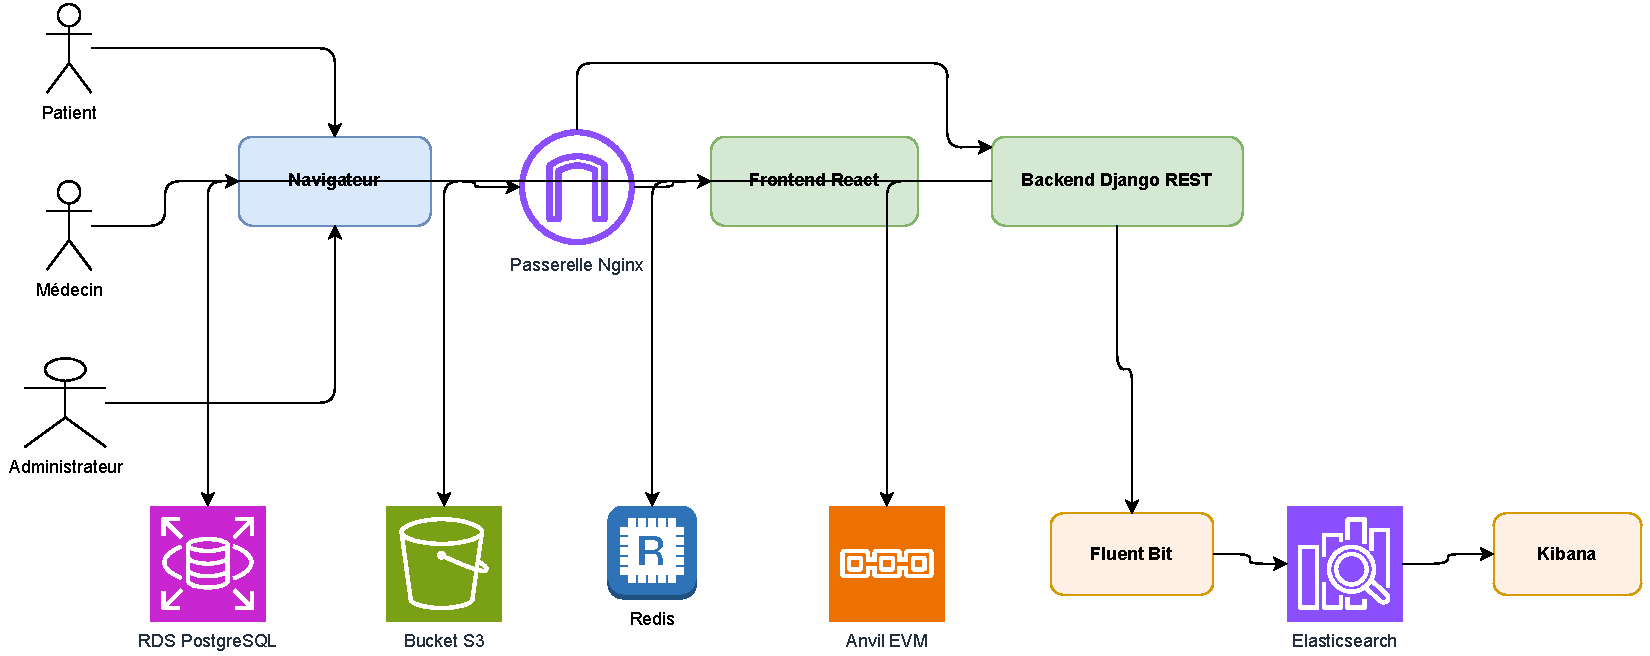
\includegraphics[width=\textwidth]{01-contexte-systeme.pdf}
\caption{Vue d'ensemble du système MedChain}
\label{fig:contexte}
\end{figure}

Les fonctionnalités principales sont :

\begin{itemize}
    \item l'authentification par jeton de session et l'authentification Google (web et mobile) ;
    \item la distinction des rôles patient, médecin et administrateur ;
    \item la gestion des rendez-vous et des dossiers médicaux ;
    \item la demande, l'activation, l'échec ou la clôture d'un épisode de traitement ;
    \item le chiffrement des événements cliniques par une clé de données propre à l'épisode ;
    \item l'ancrage des empreintes de blocs sur une chaîne EVM locale ;
    \item la supervision des comptes, des journaux d'audit et des alertes de sécurité.
\end{itemize}

\section{Étude de l'existant}

\subsection{Dossiers médicaux classiques}

Les systèmes de gestion de dossiers médicaux offrent généralement le stockage structuré des consultations, des prescriptions et des résultats d'analyses. Leurs limites sont la centralisation des données et l'absence de preuve d'intégrité indépendante du système lui-même.

\subsection{Registres distribués et ancrage}

Les registres distribués permettent de publier une empreinte immuable d'un document sans publier le document lui-même. Cette propriété est adaptée au domaine médical : on conserve le contenu chiffré dans la base et on ancre uniquement son empreinte. MedChain adopte ce modèle avec une chaîne EVM locale (Anvil) pour la phase de démonstration.

\subsection{Synthèse}

\begin{table}[H]
\centering
\renewcommand{\arraystretch}{1.3}
\begin{tabular}{|l|p{4cm}|p{4cm}|}
\hline
\textbf{Critère} & \textbf{Système classique} & \textbf{MedChain} \\
\hline
Confidentialité & Accès contrôlé & Chiffrement par épisode \\
\hline
Intégrité & Journal interne & Chaîne de blocs et ancrage \\
\hline
Traçabilité & Journaux applicatifs & Journaux + événements immuables \\
\hline
Stockage & Base unique & RDS pour les données, S3 pour les médias \\
\hline
\end{tabular}
\caption{Comparaison des approches}
\end{table}

\section{Méthodologie de travail}

Nous adoptons la méthode \textbf{Scrum}, organisée en sprints courts. Les rôles sont le Product Owner, le Scrum Master et l'équipe de développement. Les événements sont le Sprint Planning, le Daily Scrum, la revue de sprint et la rétrospective.

Les phases de réalisation retenues sont :

\begin{enumerate}
    \item analyse et spécification des besoins ;
    \item modélisation UML et conception de l'architecture ;
    \item authentification et gestion des utilisateurs ;
    \item parcours de soins et traçabilité des traitements ;
    \item sécurité, chiffrement et ancrage blockchain ;
    \item déploiement conteneurisé et validation.
\end{enumerate}

\section{Conclusion}

Ce chapitre a posé le contexte de sécurité médicale, la problématique d'intégrité et la solution proposée. Le chapitre suivant détaille les besoins fonctionnels et non fonctionnels ainsi que les modèles qui structurent l'application.

\chapter{Analyse et spécification des besoins}\label{chap2}

\section{Introduction}

Ce chapitre présente les acteurs, les besoins fonctionnels et non fonctionnels, puis les modèles qui décrivent la structure et le comportement de MedChain. Les diagrammes ont été produits au format draw.io et exportés en PDF vectoriel pour une insertion de qualité dans le rapport.

\section{Identification des acteurs}

Trois acteurs principaux interagissent avec la plateforme :

\begin{itemize}
    \item \textbf{Patient :} il consulte ses dossiers, demande un traitement, consulte la timeline de suivi et vérifie l'état d'intégrité de ses données.
    \item \textbf{Médecin :} il consulte les patients qui le concernent, gère les épisodes de traitement, ajoute des phases et des événements cliniques, et vérifie l'intégrité des chaînes de blocs.
    \item \textbf{Administrateur :} il gère les comptes et les rôles, consulte le tableau de bord de supervision, les journaux d'audit et les alertes de sécurité.
\end{itemize}

La Figure \ref{fig:use_case} résume les cas d'utilisation globaux.

\begin{figure}[H]
\centering
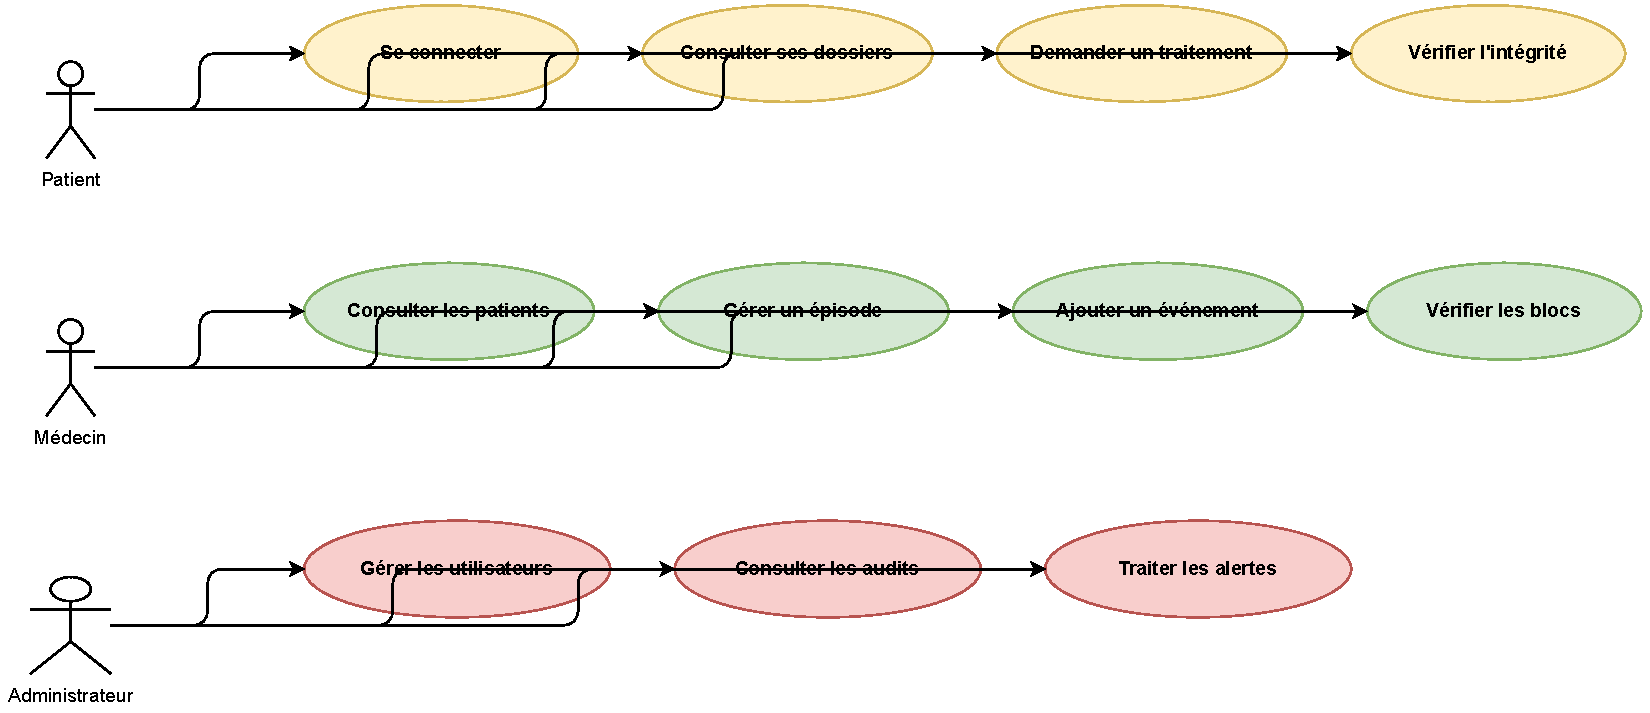
\includegraphics[width=\textwidth]{02-cas-utilisation-global.pdf}
\caption{Diagramme de cas d'utilisation global}
\label{fig:use_case}
\end{figure}

\section{Besoins fonctionnels}

\subsection{Patient}

\begin{itemize}
    \item Créer un compte, se connecter et modifier son profil.
    \item Consulter la liste des médecins et prendre rendez-vous.
    \item Consulter ses dossiers médicaux.
    \item Demander un épisode de traitement et l'abandonner si nécessaire.
    \item Consulter la timeline de traitement et les détails d'intégrité.
\end{itemize}

\subsection{Médecin}

\begin{itemize}
    \item Consulter uniquement les épisodes de traitement dont il est le médecin.
    \item Activer un épisode demandé ou le clôturer.
    \item Créer des phases de traitement et ajouter des événements cliniques.
    \item Consulter l'état de vérification des blocs et des ancres.
\end{itemize}

\subsection{Administrateur}

\begin{itemize}
    \item Créer des utilisateurs, modifier leur rôle et activer ou désactiver un compte.
    \item Forcer la déconnexion d'un utilisateur.
    \item Consulter les indicateurs du tableau de bord.
    \item Consulter les journaux d'audit et traiter les alertes de sécurité.
\end{itemize}

\section{Besoins non fonctionnels}

\begin{itemize}
    \item \textbf{Confidentialité :} les charges utiles des événements cliniques sont chiffrées avec AES-GCM avant stockage.
    \item \textbf{Intégrité :} toute tentative de modification d'un bloc est rejetée ; les empreintes sont ancrées sur une chaîne EVM.
    \item \textbf{Traçabilité :} les connexions, consultations et refus d'accès sont enregistrés dans \texttt{AuditLog}.
    \item \textbf{Moindre privilège :} les requêtes sont filtrées selon le rôle et l'appartenance des données.
    \item \textbf{Disponibilité :} les services sont conteneurisés et supervisés par des healthchecks.
    \item \textbf{Maintenabilité :} la configuration sensible est externalisée dans l'environnement.
    \item \textbf{Sécurité des dépendances :} les versions sont épinglées dans \texttt{requirements.txt}.
\end{itemize}

\section{Modèle de domaine}

La Figure \ref{fig:domain} présente les entités principales et leurs relations. Le cœur du modèle est l'épisode de traitement, auquel sont rattachés les phases, les événements cliniques, les blocs, la clé encapsulée et les ancres.

\begin{figure}[H]
\centering
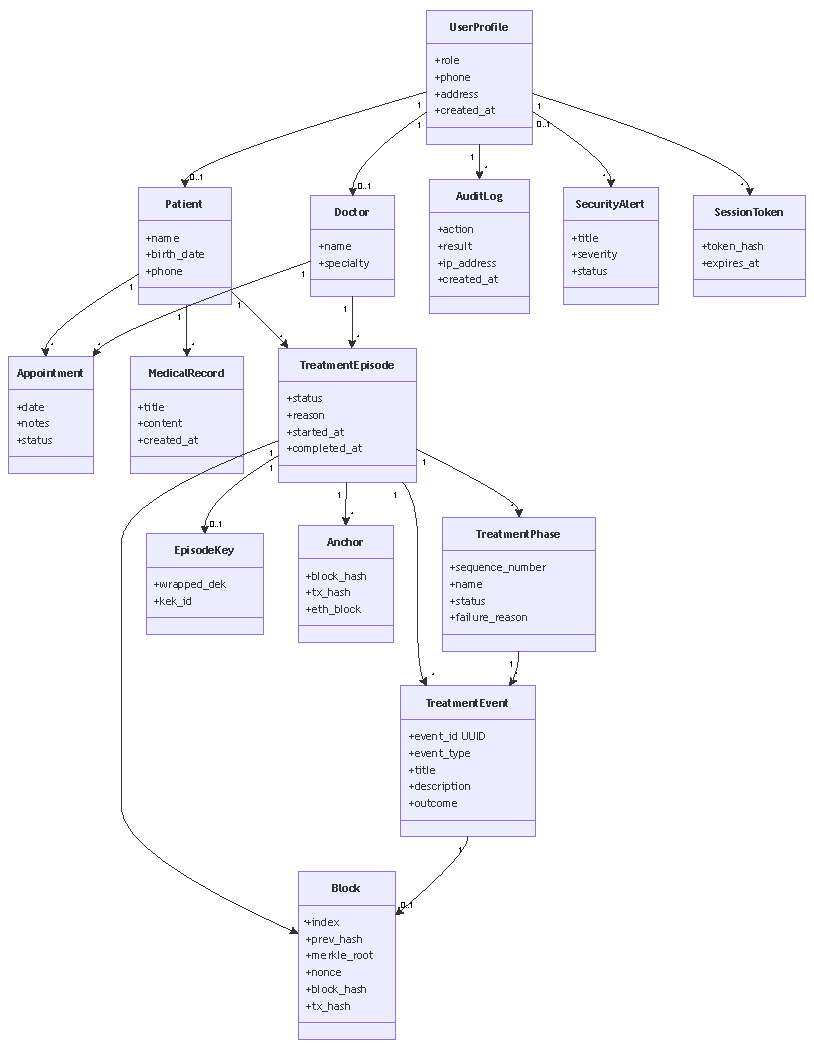
\includegraphics[width=\textwidth]{05-modele-de-domaine.pdf}
\caption{Diagramme de classes du modèle de domaine}
\label{fig:domain}
\end{figure}

\section{Architecture logicielle}

La Figure \ref{fig:backend_arch} décrit l'organisation en couches du backend : le middleware et le routage, les vues d'authentification, les vues métier et d'administration, les sérialiseurs, les modèles puis les services de stockage, de chiffrement et de journalisation.

\begin{figure}[H]
\centering
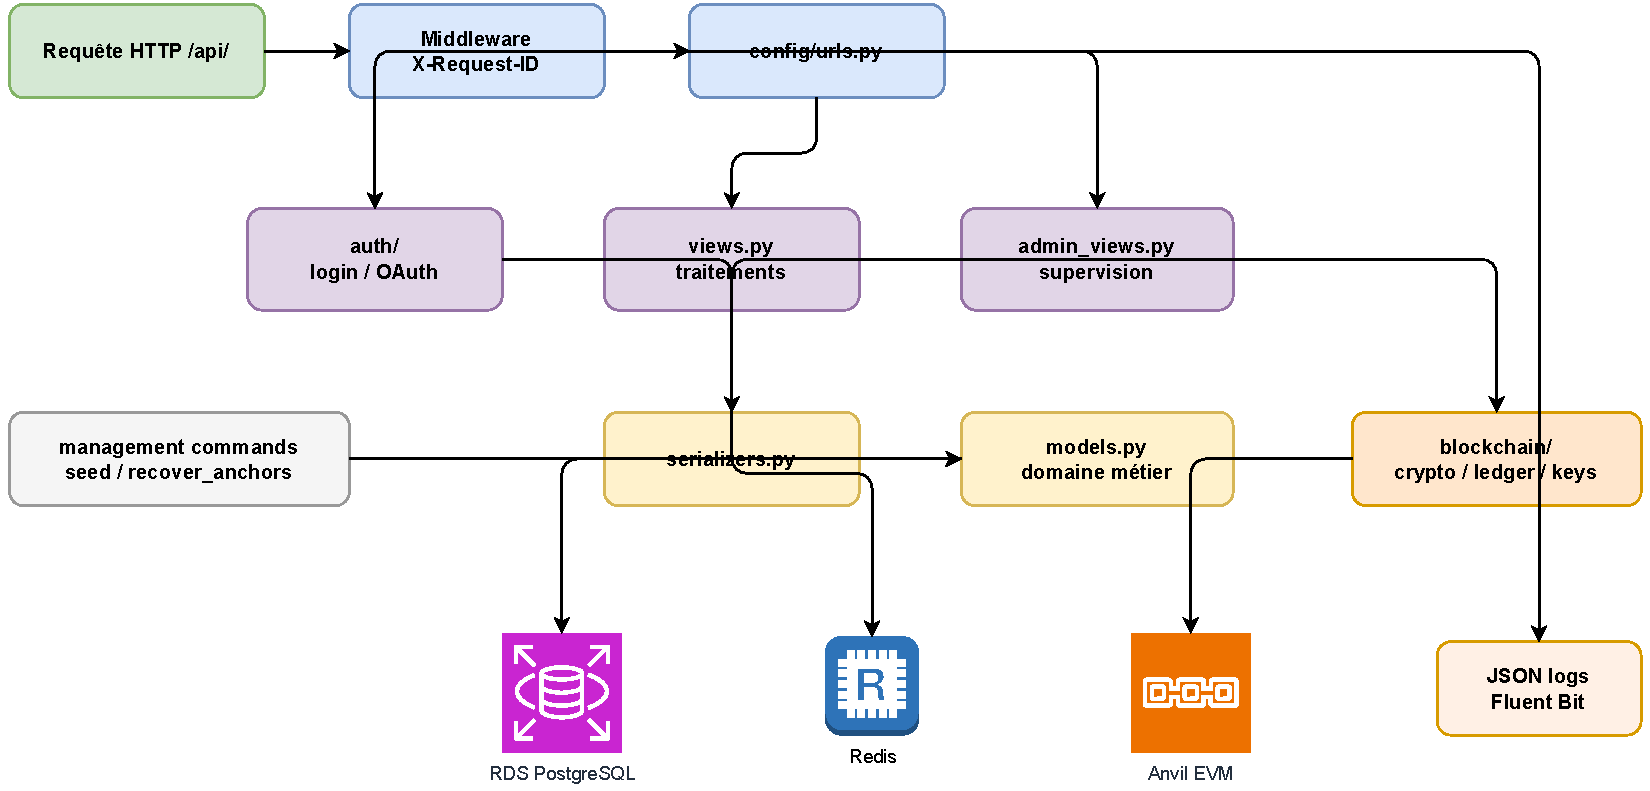
\includegraphics[width=\textwidth]{04-architecture-backend.pdf}
\caption{Architecture en couches du backend}
\label{fig:backend_arch}
\end{figure}

La Figure \ref{fig:frontend_arch} décrit l'application monopage : les fournisseurs de contexte, le routeur, les pages publiques et protégées, puis la couche de services HTTP qui communique avec la passerelle.

\begin{figure}[H]
\centering
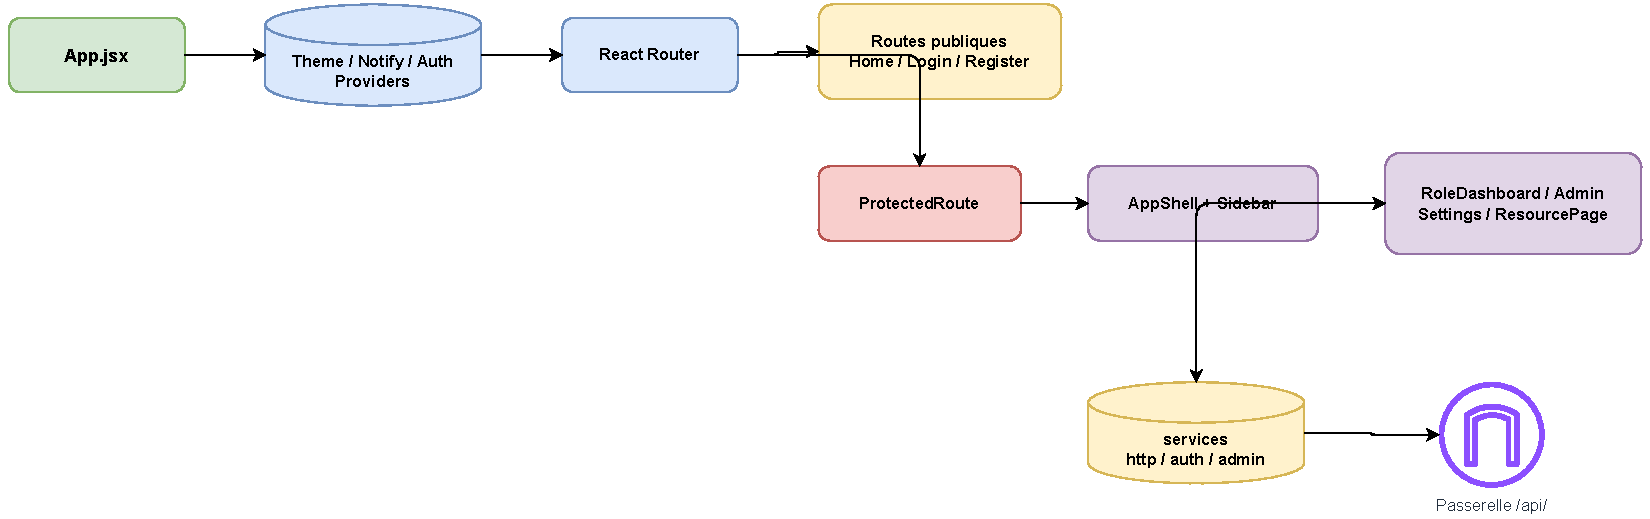
\includegraphics[width=\textwidth]{12-architecture-frontend.pdf}
\caption{Architecture de l'application frontend}
\label{fig:frontend_arch}
\end{figure}

\section{Conclusion}

Les besoins et les modèles étant établis, les chapitres suivants détaillent les sprints de réalisation : authentification, parcours de soins, puis sécurité et déploiement.

\chapter{Sprint 1 : Authentification et gestion des utilisateurs}\label{chap4}

\section{Introduction}

Le premier sprint est consacré à l'identification des utilisateurs et au contrôle d'accès. L'objectif est de permettre l'inscription, la connexion par jeton de session, l'authentification Google et la gestion des profils selon trois rôles.

\section{Objectifs du sprint}

\begin{itemize}
    \item Mettre en place l'inscription et la connexion sécurisée.
    \item Générer un jeton de session stocké sous forme de hash dans la base.
    \item Intégrer Google OAuth pour le web et le mobile.
    \item Distinguer les rôles patient, médecin et administrateur.
    \item Réaliser les interfaces de connexion, d'inscription et de paramètres.
\end{itemize}

\section{Backlog du sprint}

\begin{table}[H]
\centering
\begin{tabular}{|p{3cm}|p{6cm}|p{2cm}|p{3cm}|}
\hline
\textbf{User story} & \textbf{Description} & \textbf{Priorité} & \textbf{Critère d'acceptation} \\
\hline
US1 --- Inscription & Créer un compte patient & Haute & Compte créé et profil patient associé \\
\hline
US2 --- Connexion & S'authentifier avec email et mot de passe & Haute & Jeton retourné et redirection selon le rôle \\
\hline
US3 --- Rôles & Restreindre les routes selon le rôle & Haute & Accès refusé pour un rôle non autorisé \\
\hline
US4 --- Profil & Modifier ses informations personnelles & Moyenne & Modification enregistrée \\
\hline
\end{tabular}
\caption{Backlog du sprint 1}
\end{table}

\section{Authentification par jeton}

La Figure \ref{fig:auth_seq} décrit le déroulement d'une connexion. Le mot de passe est vérifié côté backend, puis un jeton aléatoire est généré ; seul son hash SHA-256 est conservé dans \texttt{SessionToken}. Le profil utilisateur est mis en cache dans Redis pour accélérer les requêtes suivantes.

\begin{figure}[H]
\centering
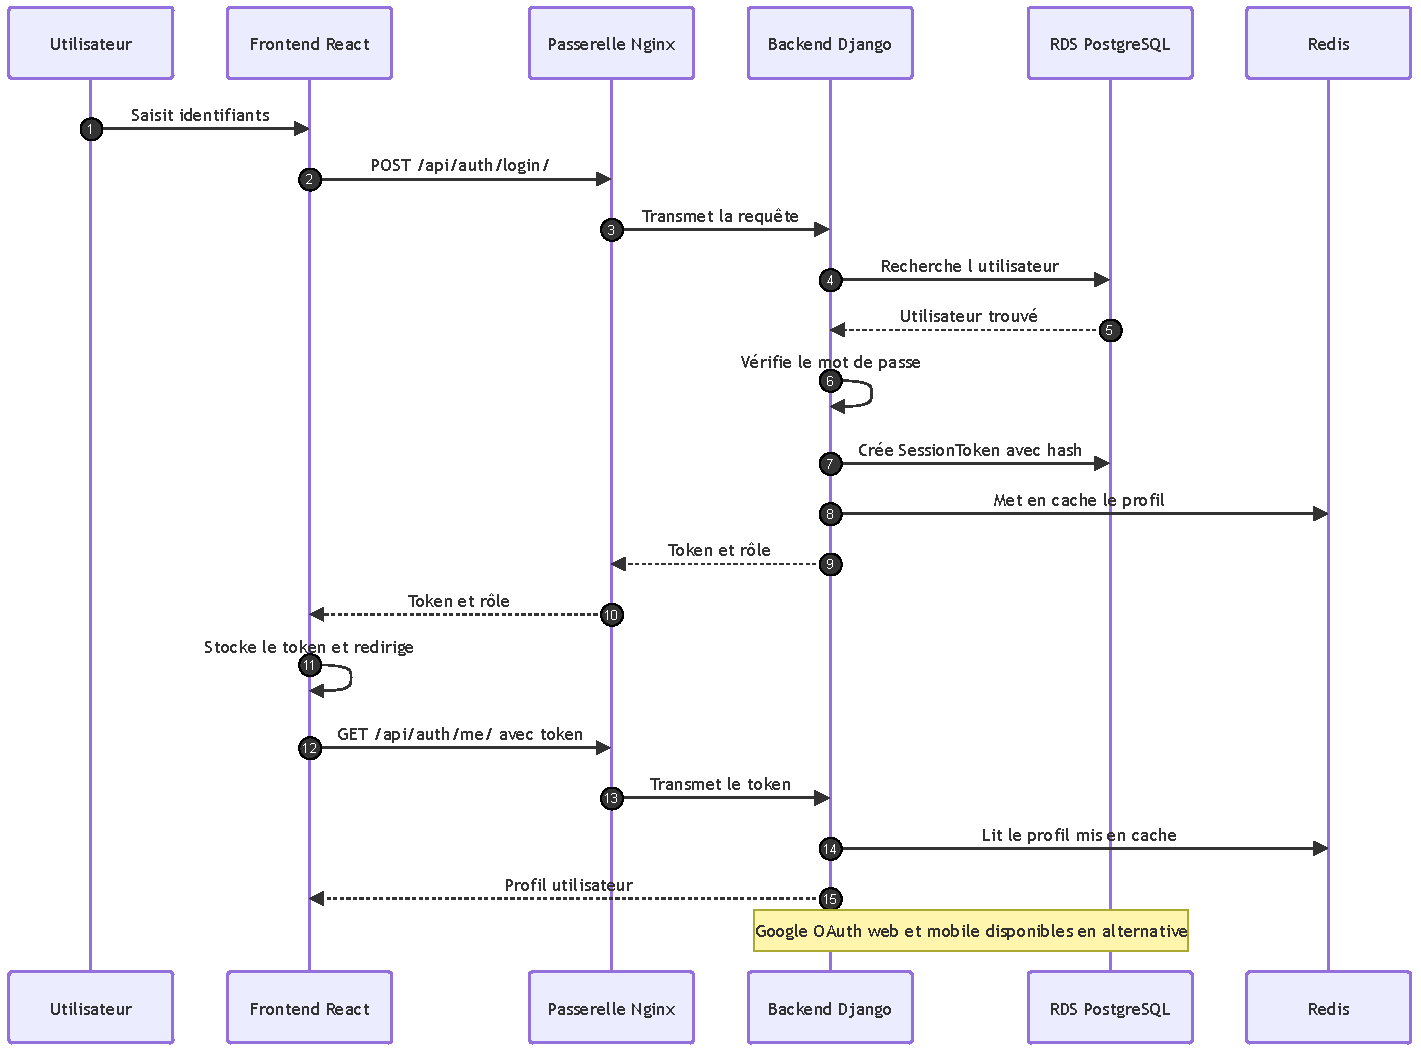
\includegraphics[width=\textwidth]{06-authentification-sequence.pdf}
\caption{Séquence d'authentification par jeton}
\label{fig:auth_seq}
\end{figure}

\section{Contrôle d'accès}

Le contrôle d'accès repose sur deux mécanismes complémentaires : la vérification du rôle pour les opérations sensibles et le filtrage des requêtes selon l'appartenance des données. Un médecin ne voit ainsi que les épisodes dont il est le praticien, et un patient uniquement les siens. Les refus sont journalisés dans \texttt{AuditLog}.

\section{Réalisation}

La Figure \ref{fig:login_screen} présente la page de connexion et la Figure \ref{fig:register_screen} la page d'inscription.

\begin{figure}[H]
\centering
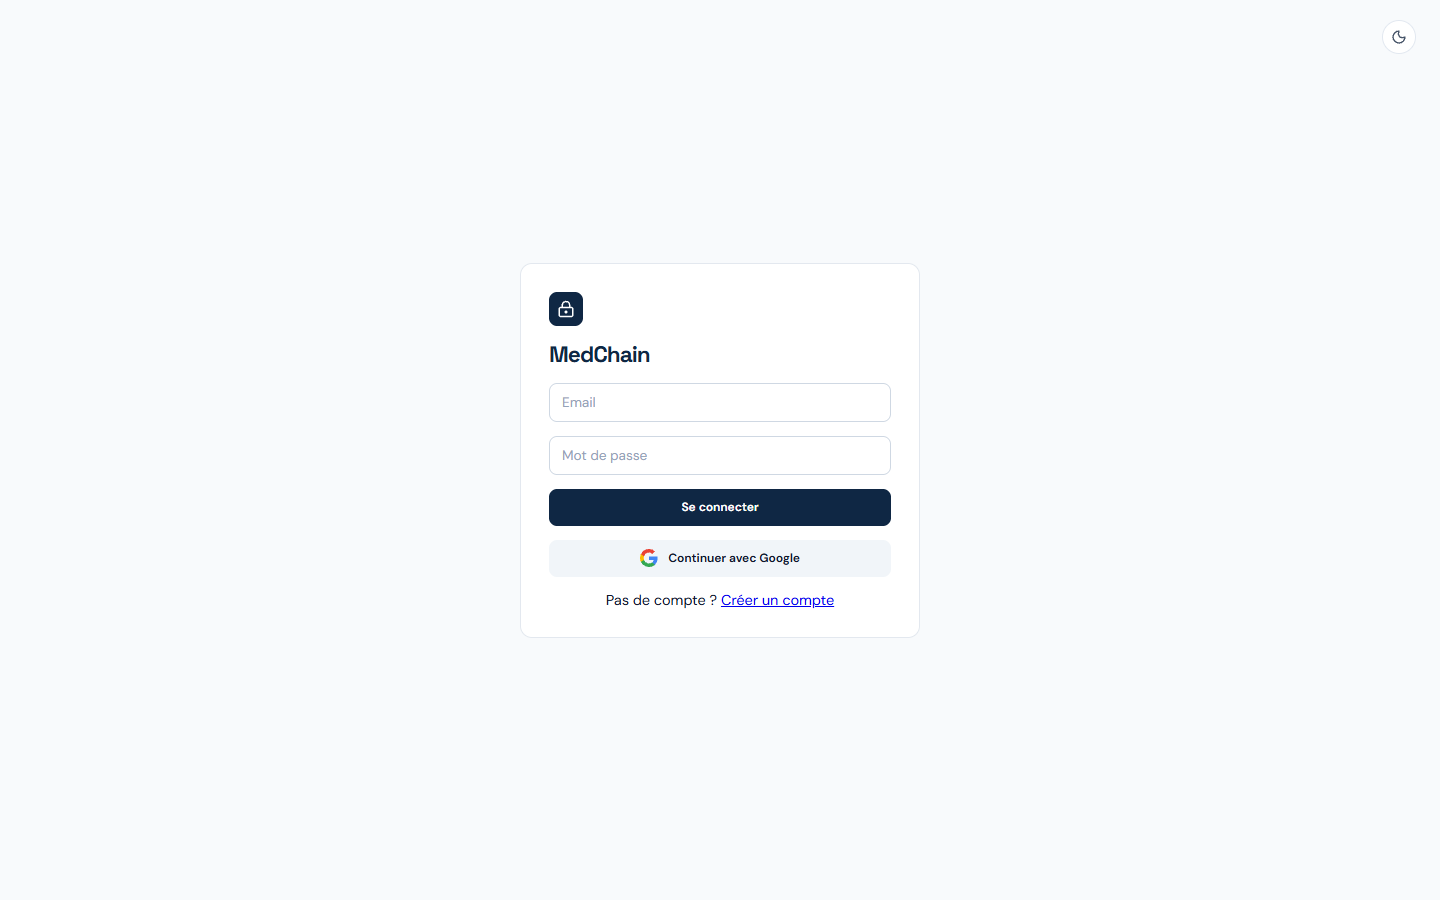
\includegraphics[width=0.8\textwidth]{S02-connexion.png}
\caption{Interface de connexion}
\label{fig:login_screen}
\end{figure}

\begin{figure}[H]
\centering
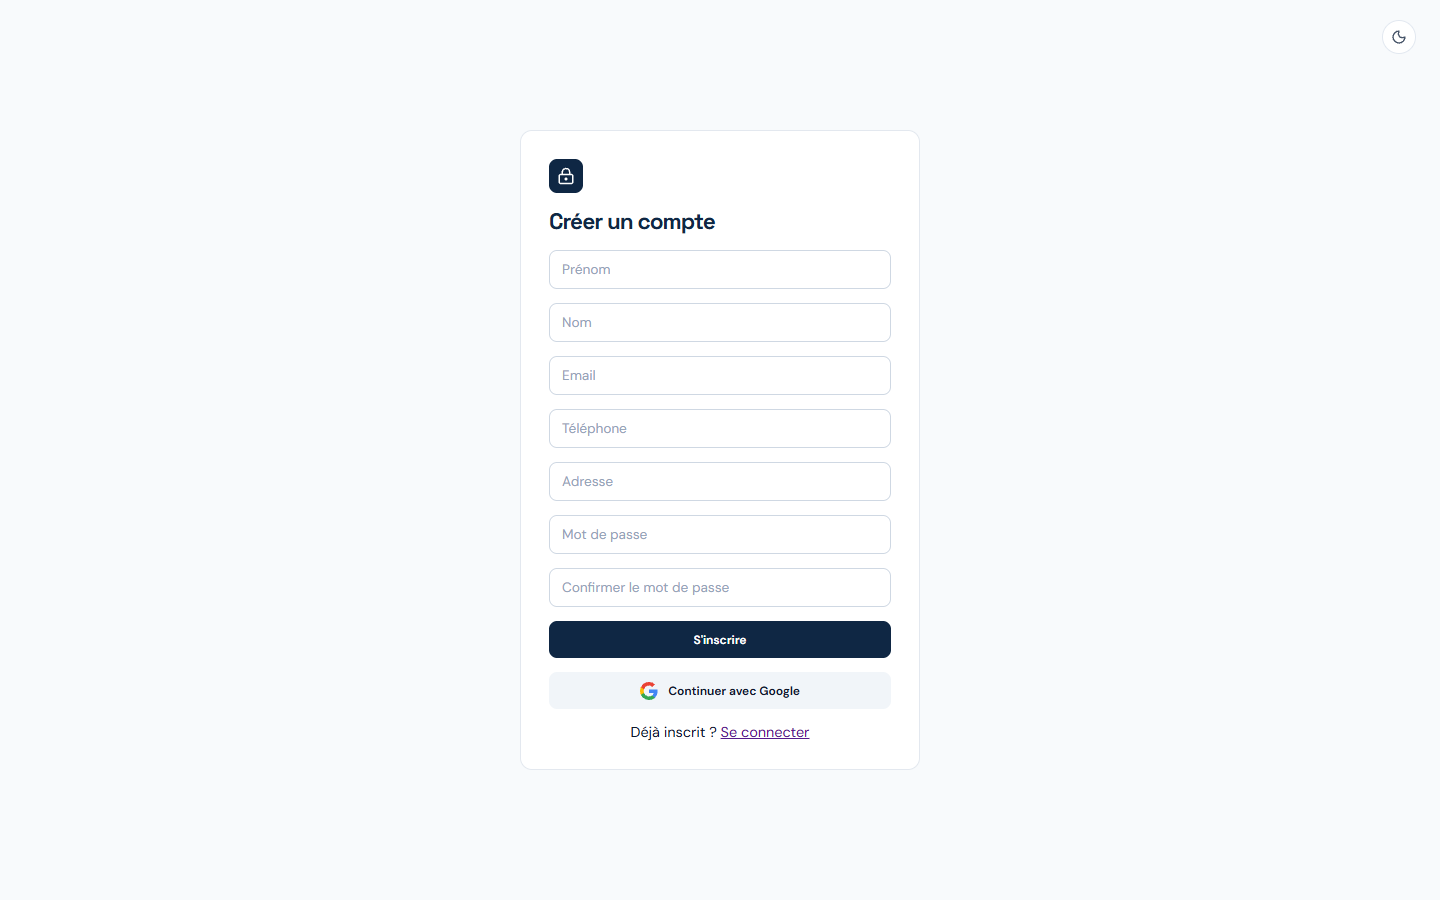
\includegraphics[width=0.8\textwidth]{S03-inscription.png}
\caption{Interface d'inscription}
\label{fig:register_screen}
\end{figure}

La Figure \ref{fig:settings_screen} montre la page de paramètres du compte et la Figure \ref{fig:admin_screen} le tableau de bord réservé à l'administrateur.

\begin{figure}[H]
\centering
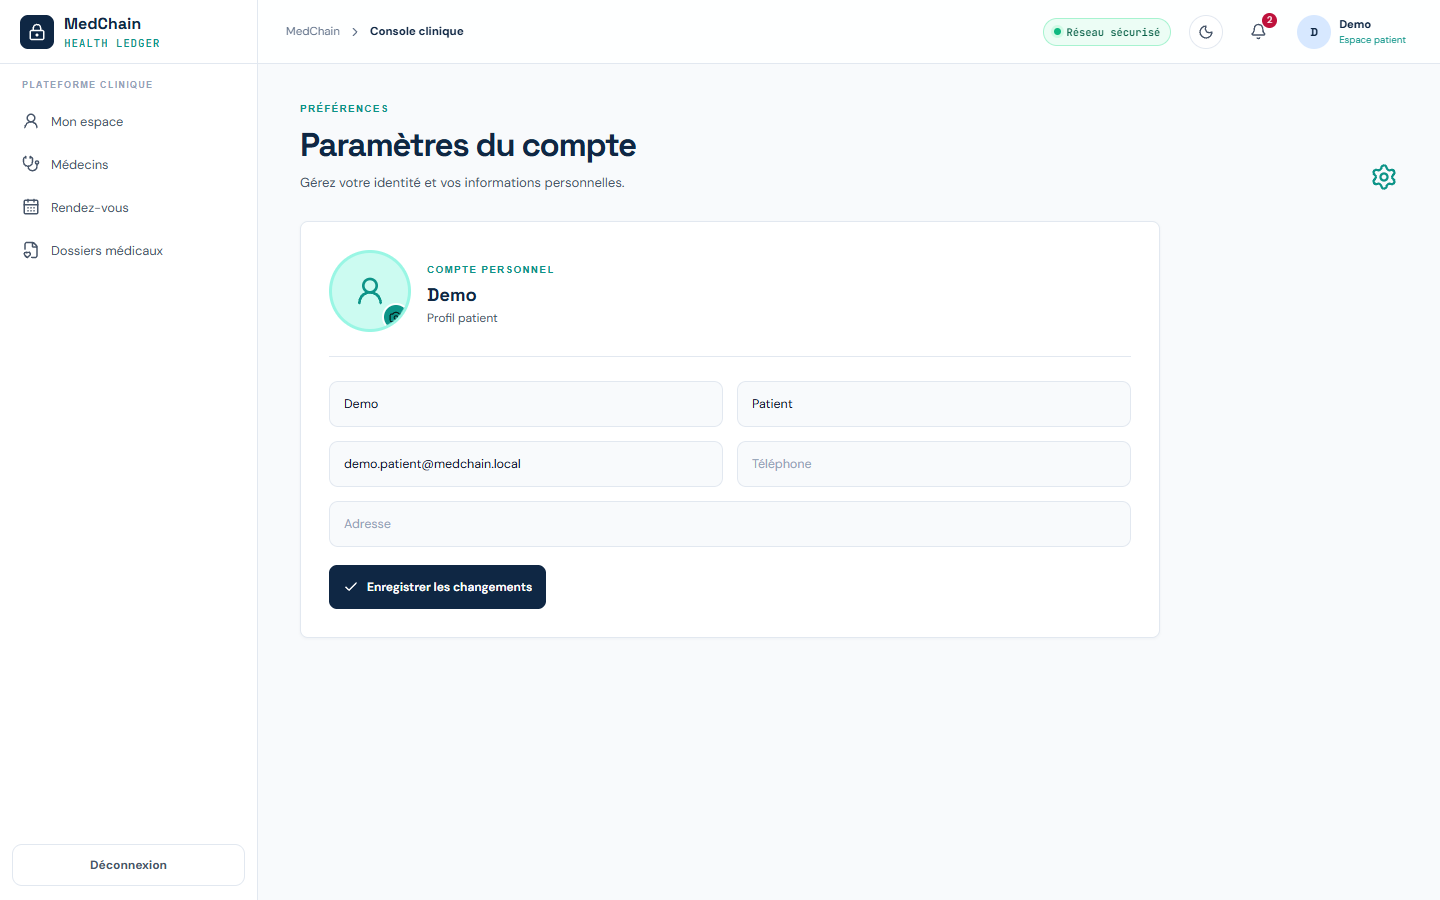
\includegraphics[width=\textwidth]{S10-parametres.png}
\caption{Paramètres du compte}
\label{fig:settings_screen}
\end{figure}

\begin{figure}[H]
\centering
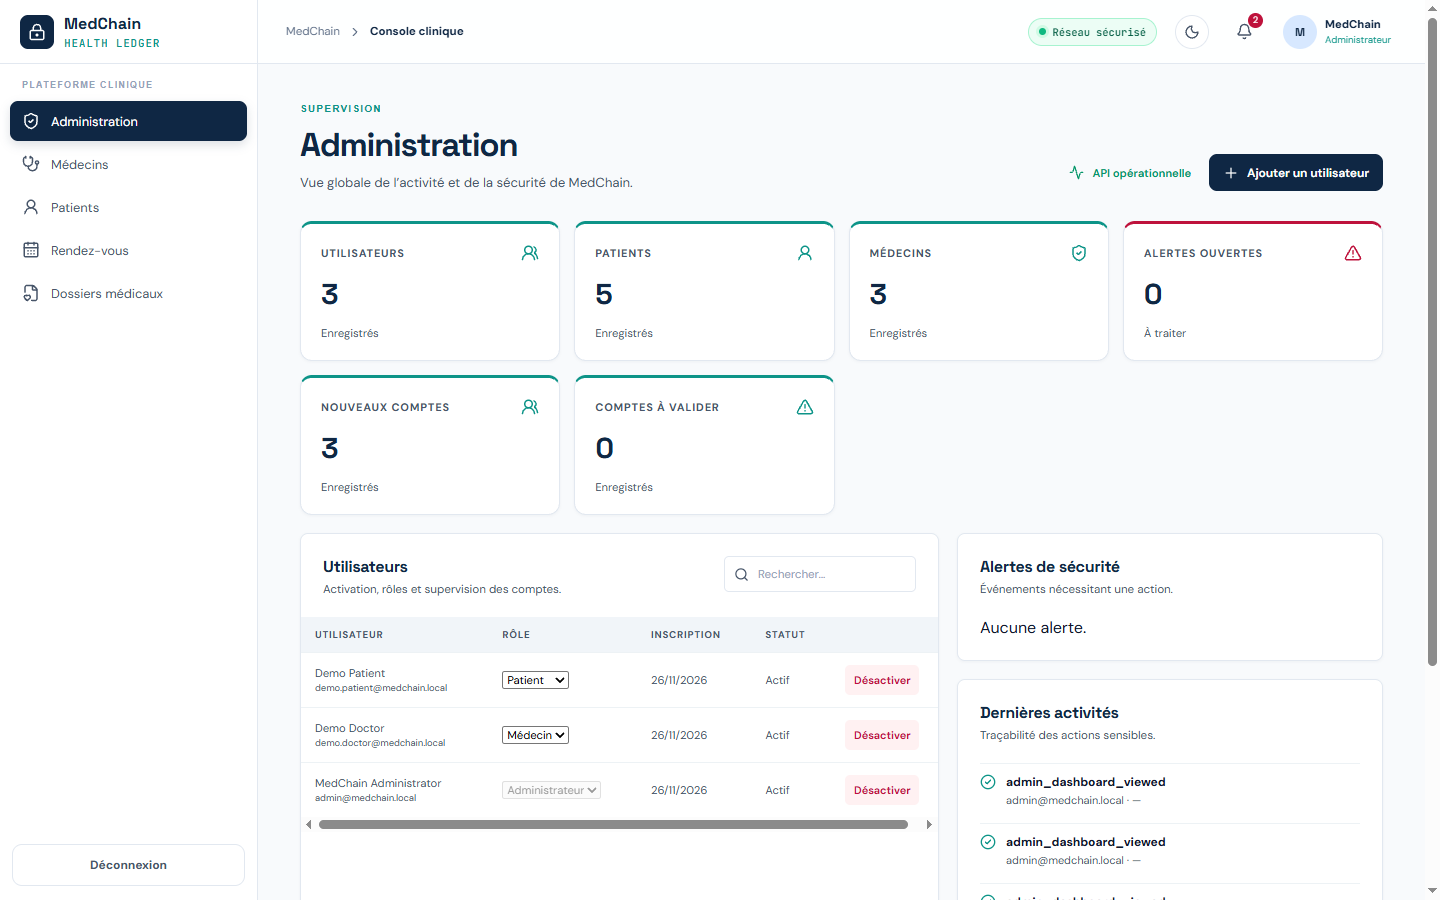
\includegraphics[width=\textwidth]{S14-tableau-administrateur.png}
\caption{Tableau de bord administrateur}
\label{fig:admin_screen}
\end{figure}

\section{Conclusion}

À l'issue de ce sprint, l'authentification, la gestion des rôles et la supervision des comptes sont opérationnelles. Le sprint suivant porte sur le parcours de soins et la traçabilité des traitements.

\chapter{Sprint 2 : Parcours de soins et traçabilité}\label{chap5}

\section{Introduction}

Le deuxième sprint couvre le parcours clinique : consultation des médecins et des patients, gestion des rendez-vous et des dossiers médicaux, demande et suivi d'un épisode de traitement. Il introduit également la vérification d'intégrité consultable depuis l'interface patient et médecin.

\section{Objectifs du sprint}

\begin{itemize}
    \item Permettre au patient de demander un traitement et d'abandonner un épisode en cours.
    \item Permettre au médecin d'activer ou de clôturer un épisode.
    \item Gérer les phases et les événements cliniques d'un épisode.
    \item Afficher la timeline de suivi et l'état de vérification des blocs.
    \item Fournir une interface de consultation des ressources cliniques.
\end{itemize}

\section{Contrôle d'accès au parcours de soins}

La Figure \ref{fig:access_seq} illustre le filtrage des données. Le patient demande un traitement, le médecin consulte la timeline de l'épisode, et le backend applique le filtrage selon le rôle. Lorsque l'épisode n'appartient pas à l'utilisateur, la réponse est un \texttt{403 Forbidden} et un événement \texttt{denied} est écrit dans le journal d'audit.

\begin{figure}[H]
\centering
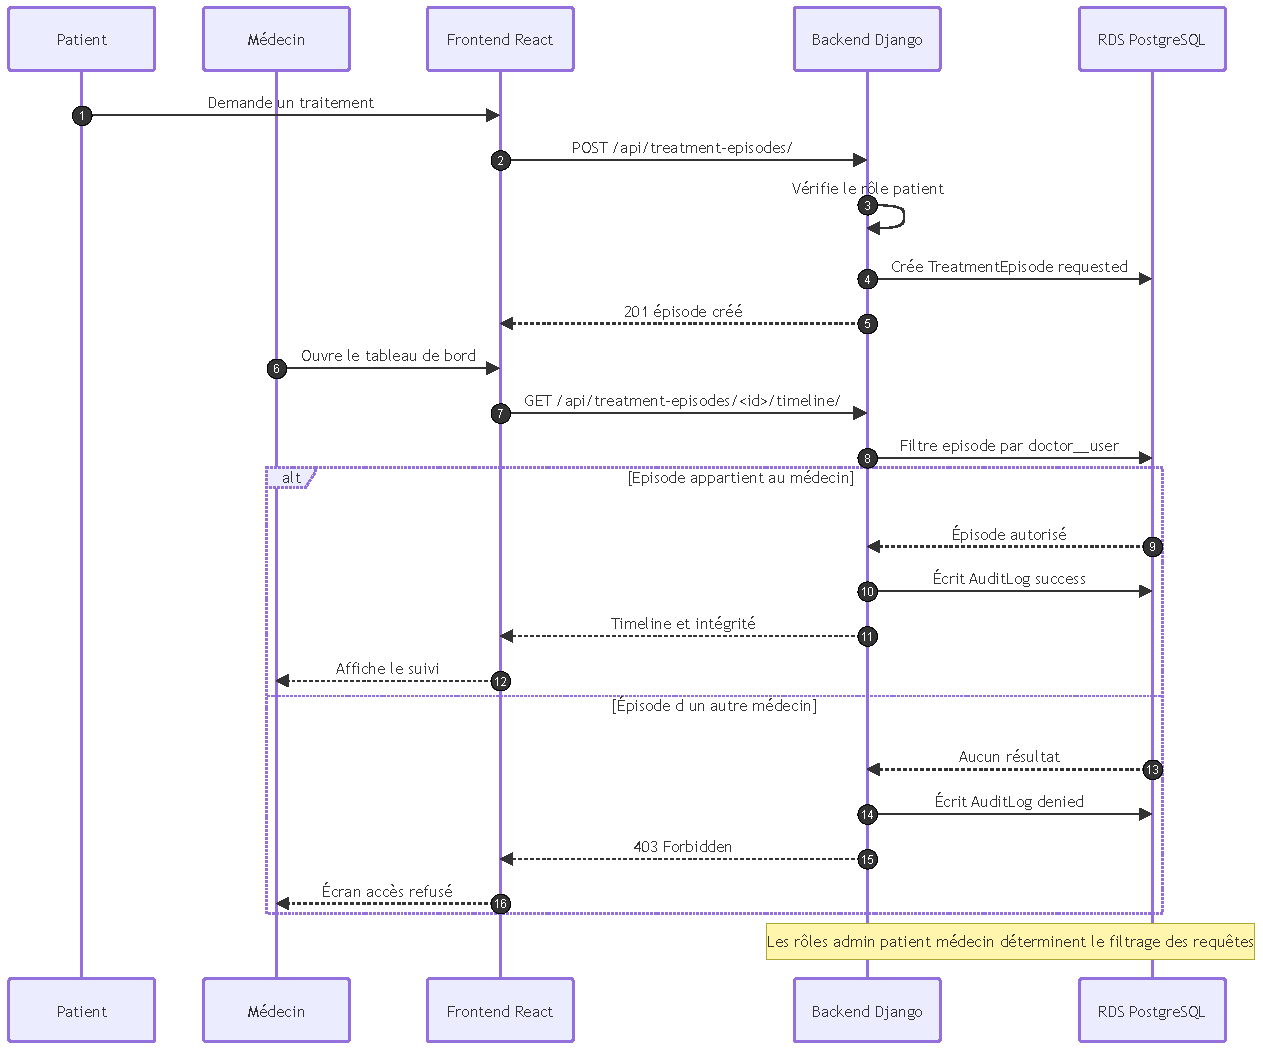
\includegraphics[width=\textwidth]{07-controle-acces-sequence.pdf}
\caption{Séquence de contrôle d'accès à un épisode}
\label{fig:access_seq}
\end{figure}

\section{Cycle de vie d'un traitement}

La Figure \ref{fig:states} décrit les états d'un épisode de traitement et ceux d'une phase. Un épisode passe de \textit{demandé} à \textit{actif} sur action du médecin, puis à \textit{terminé} ou \textit{abandonné}. Une phase peut être \textit{en attente}, \textit{active}, \textit{terminée}, \textit{échouée} ou \textit{ignorée}.

\begin{figure}[H]
\centering
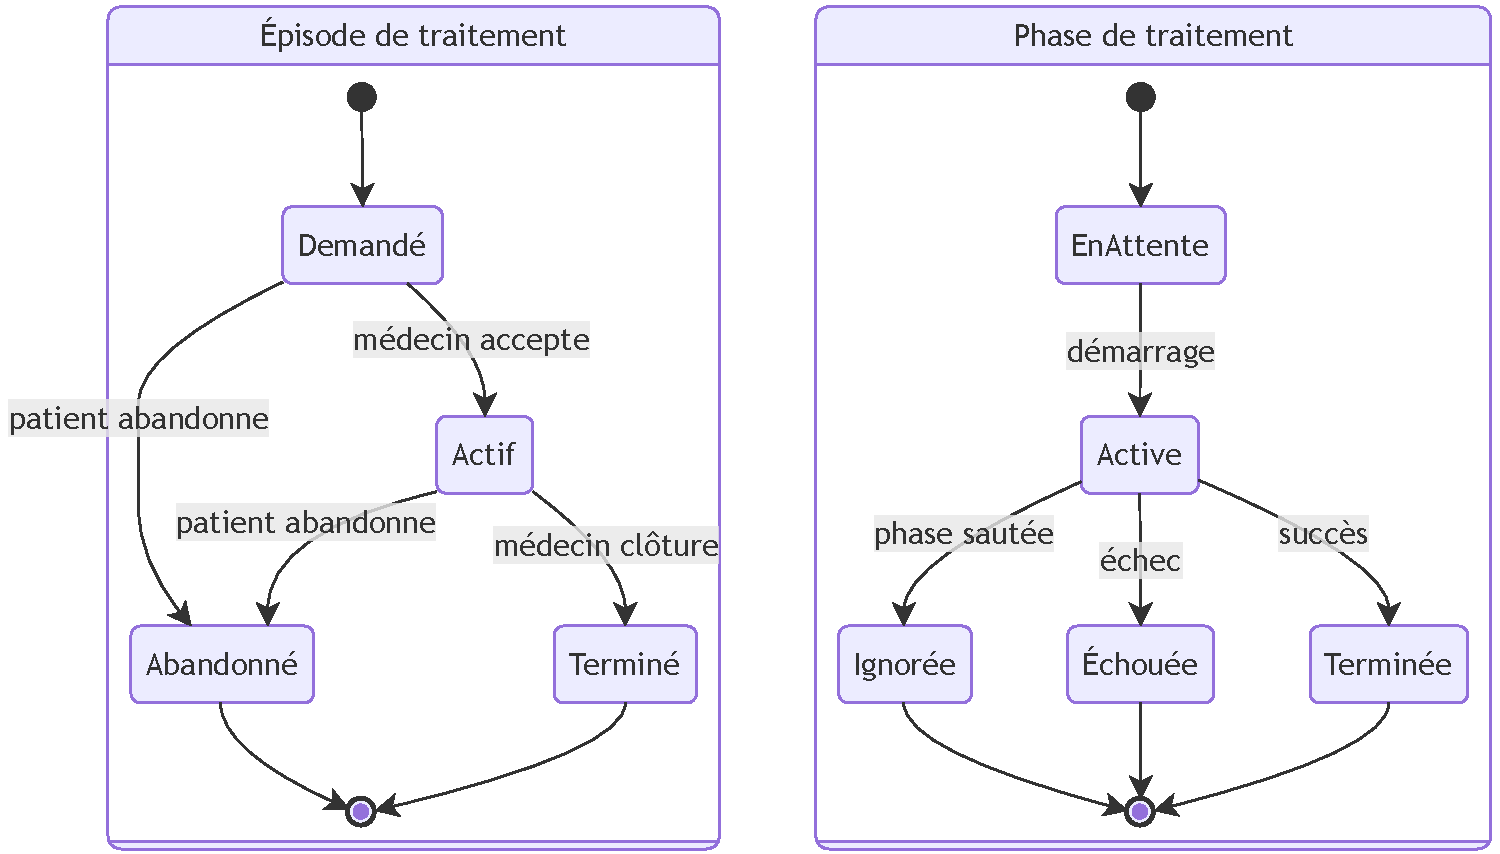
\includegraphics[width=\textwidth]{08-cycle-traitement-etats.pdf}
\caption{Diagrammes d'états du traitement}
\label{fig:states}
\end{figure}

\section{Réalisation --- Espace patient}

La Figure \ref{fig:patient_dash} présente l'espace patient avec la liste des traitements et la demande de suivi. La Figure \ref{fig:integrity} montre le panneau de détails d'intégrité, où le patient peut lire les hashs de blocs, les racines Merkle et les transactions d'ancrage.

\begin{figure}[H]
\centering
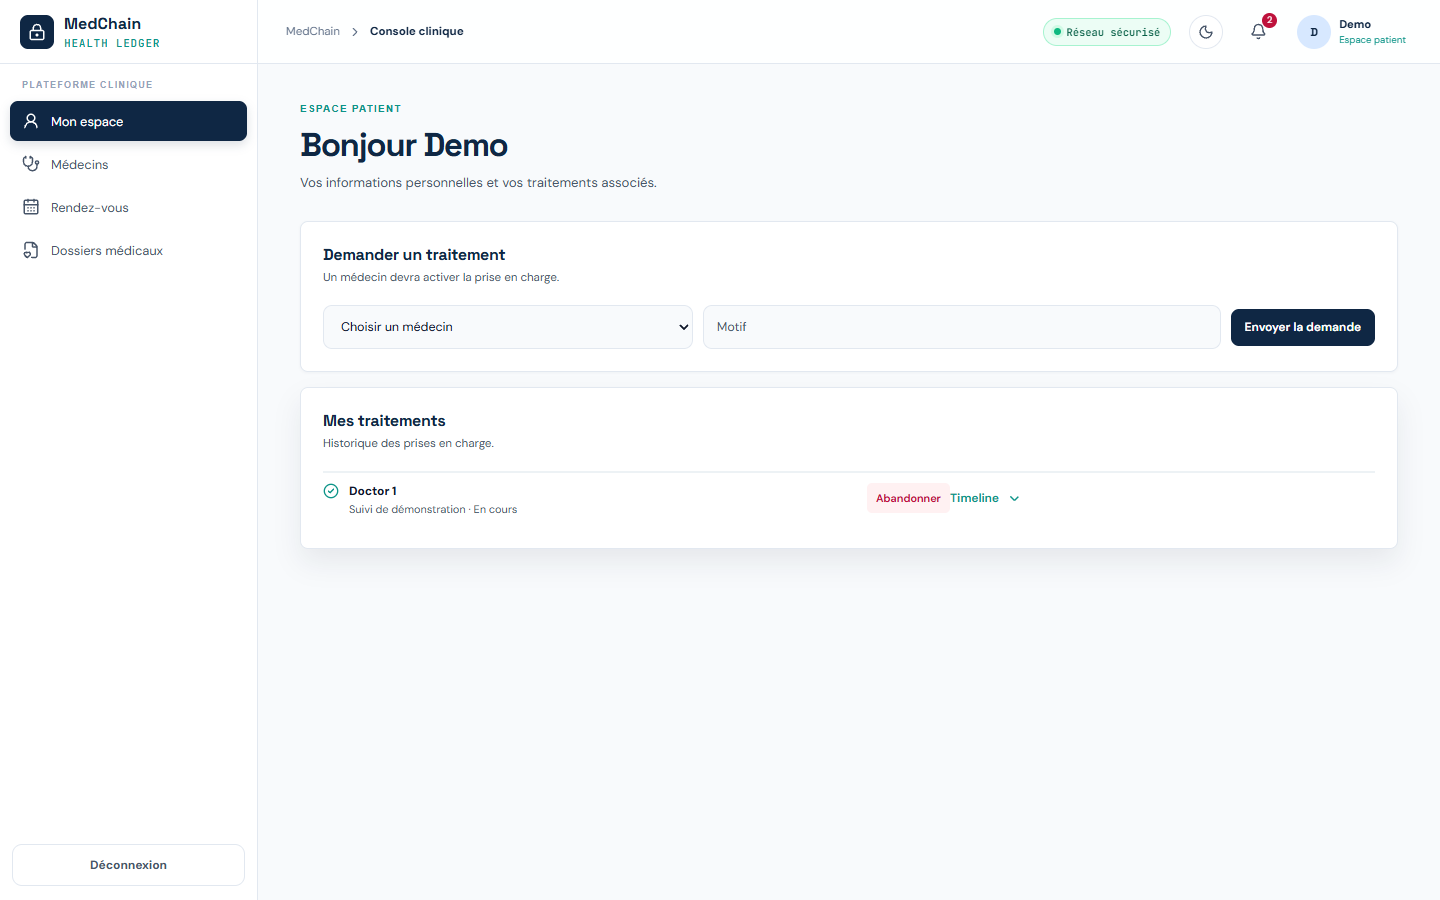
\includegraphics[width=\textwidth]{S04-espace-patient.png}
\caption{Tableau de bord patient}
\label{fig:patient_dash}
\end{figure}

\begin{figure}[H]
\centering
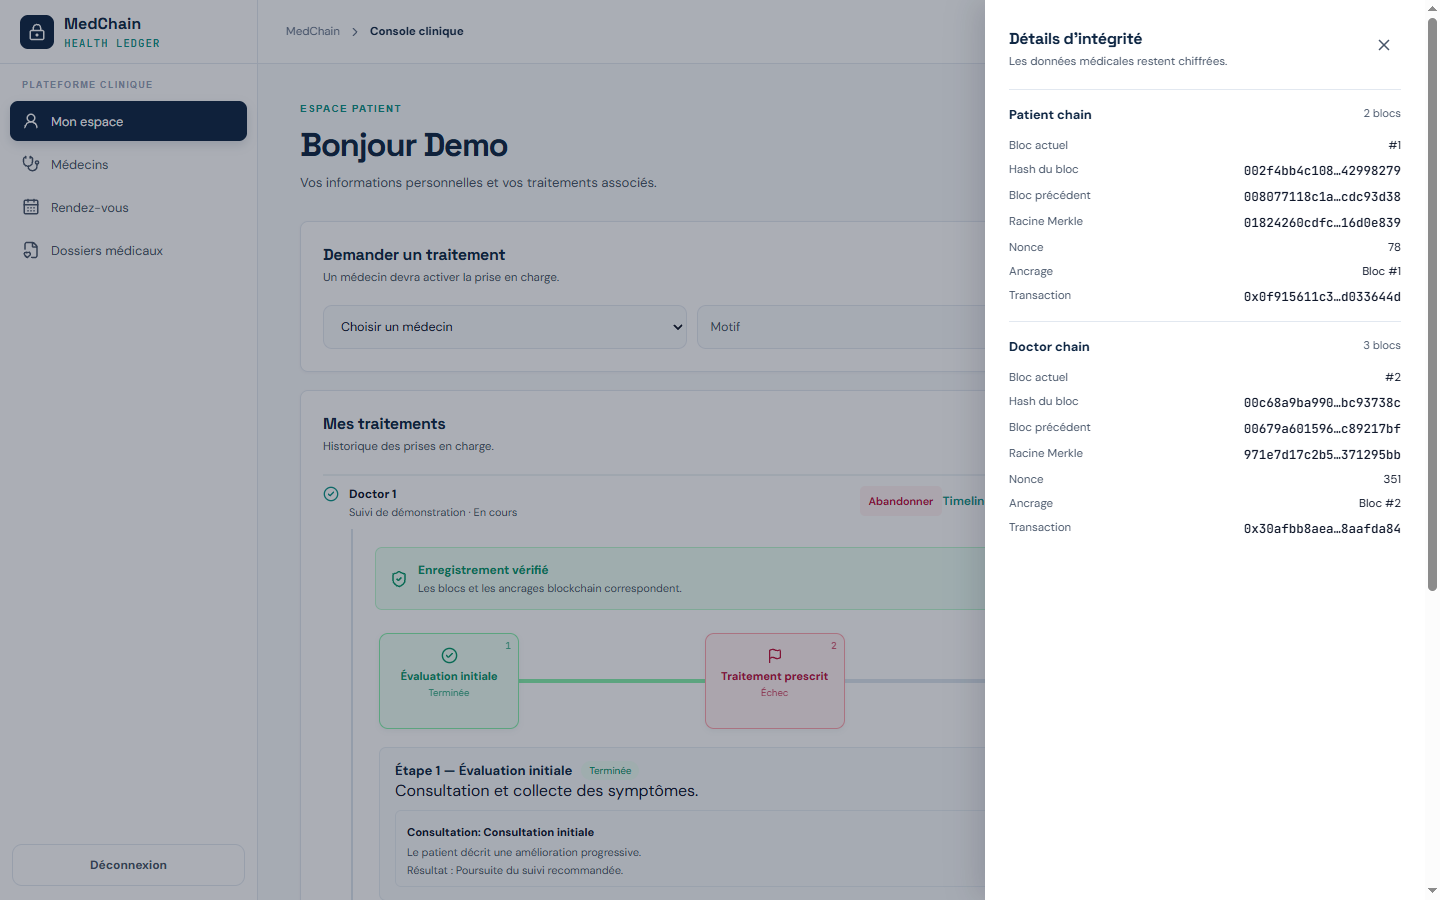
\includegraphics[width=\textwidth]{S05-details-integrite.png}
\caption{Détails d'intégrité des chaînes}
\label{fig:integrity}
\end{figure}

Les Figures \ref{fig:doctors}, \ref{fig:appointments}, \ref{fig:appointment_form} et \ref{fig:records} illustrent la gestion des ressources cliniques.

\begin{figure}[H]
\centering
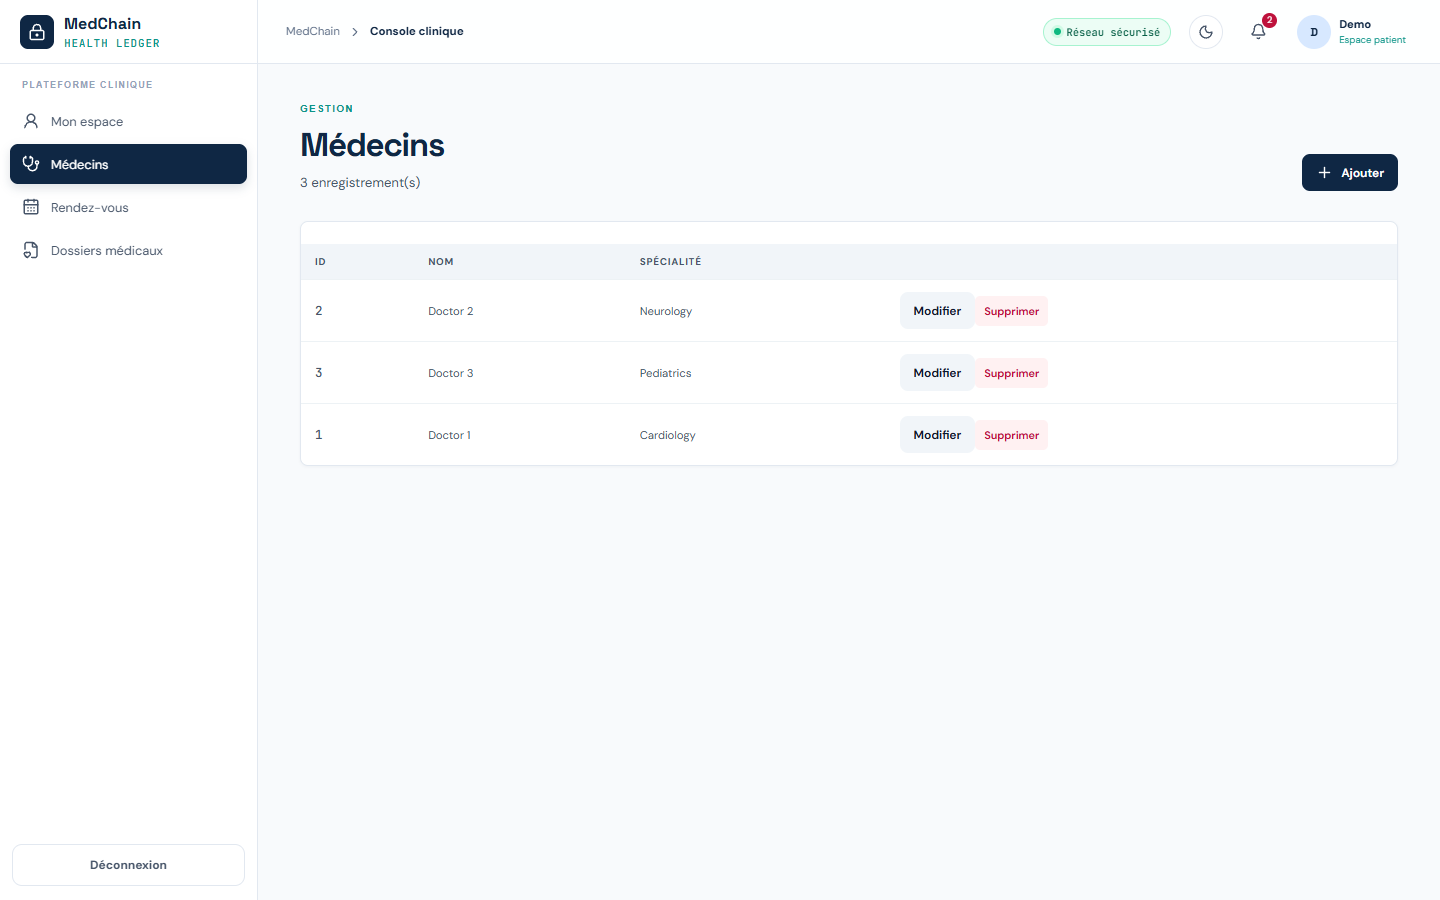
\includegraphics[width=\textwidth]{S06-liste-medecins.png}
\caption{Liste des médecins}
\label{fig:doctors}
\end{figure}

\begin{figure}[H]
\centering
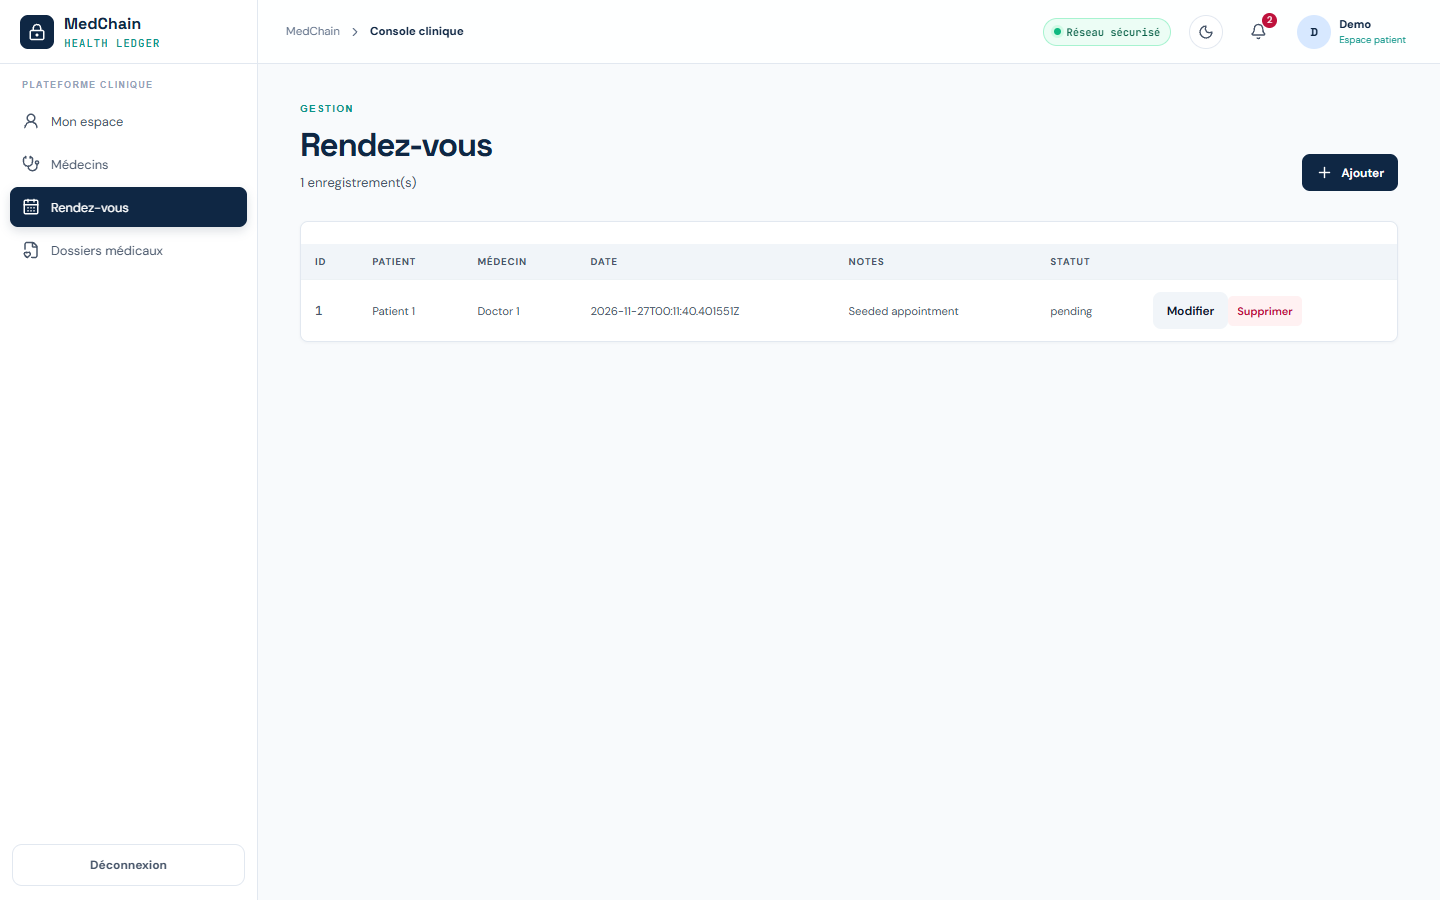
\includegraphics[width=\textwidth]{S07-liste-rendezvous.png}
\caption{Liste des rendez-vous}
\label{fig:appointments}
\end{figure}

\begin{figure}[H]
\centering
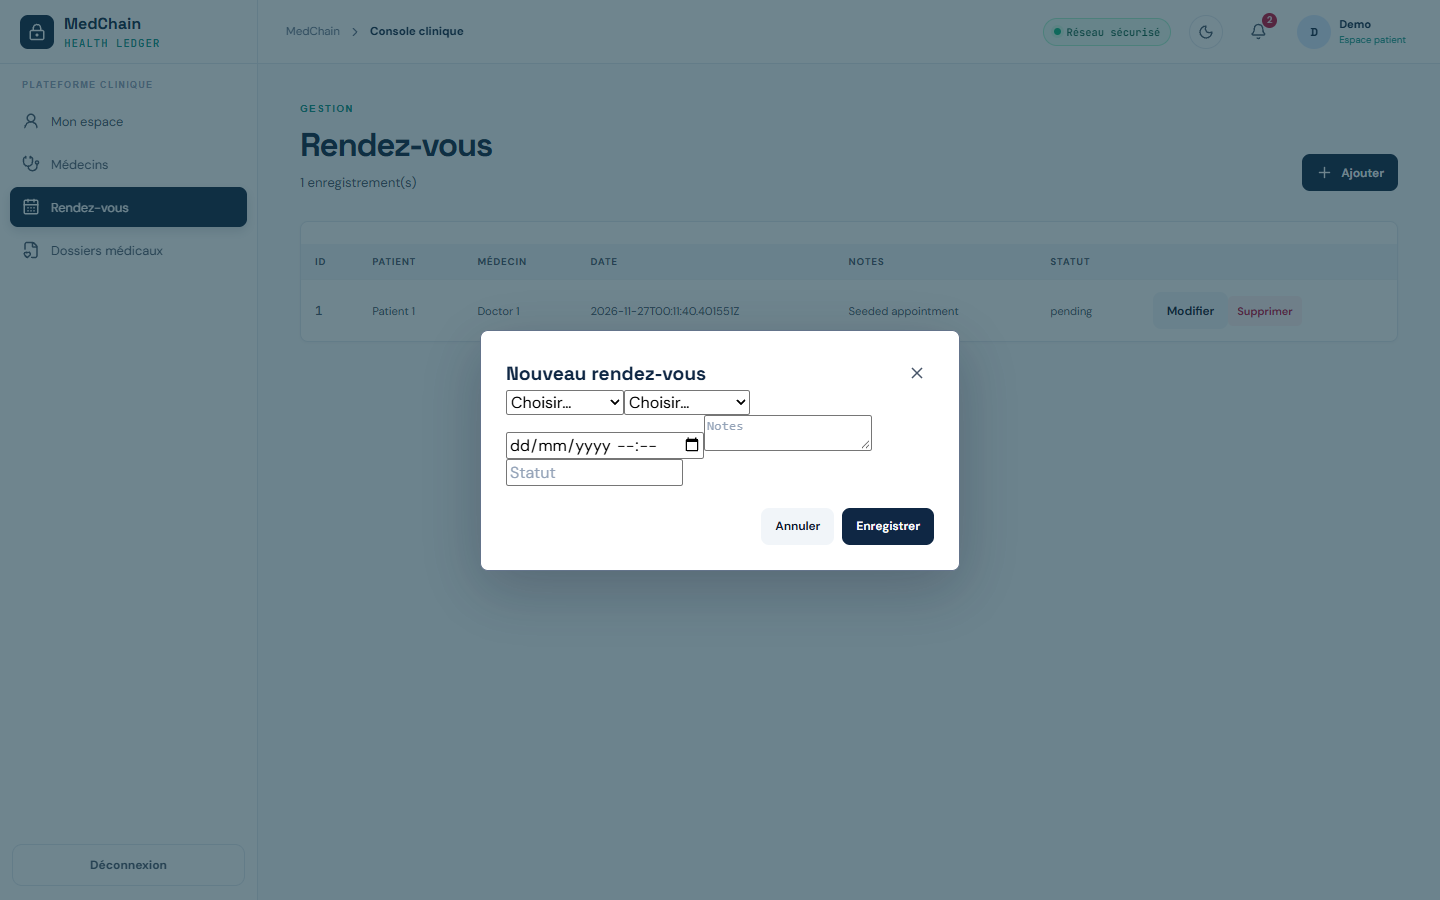
\includegraphics[width=\textwidth]{S08-creation-rendezvous.png}
\caption{Formulaire de création d'un rendez-vous}
\label{fig:appointment_form}
\end{figure}

\begin{figure}[H]
\centering
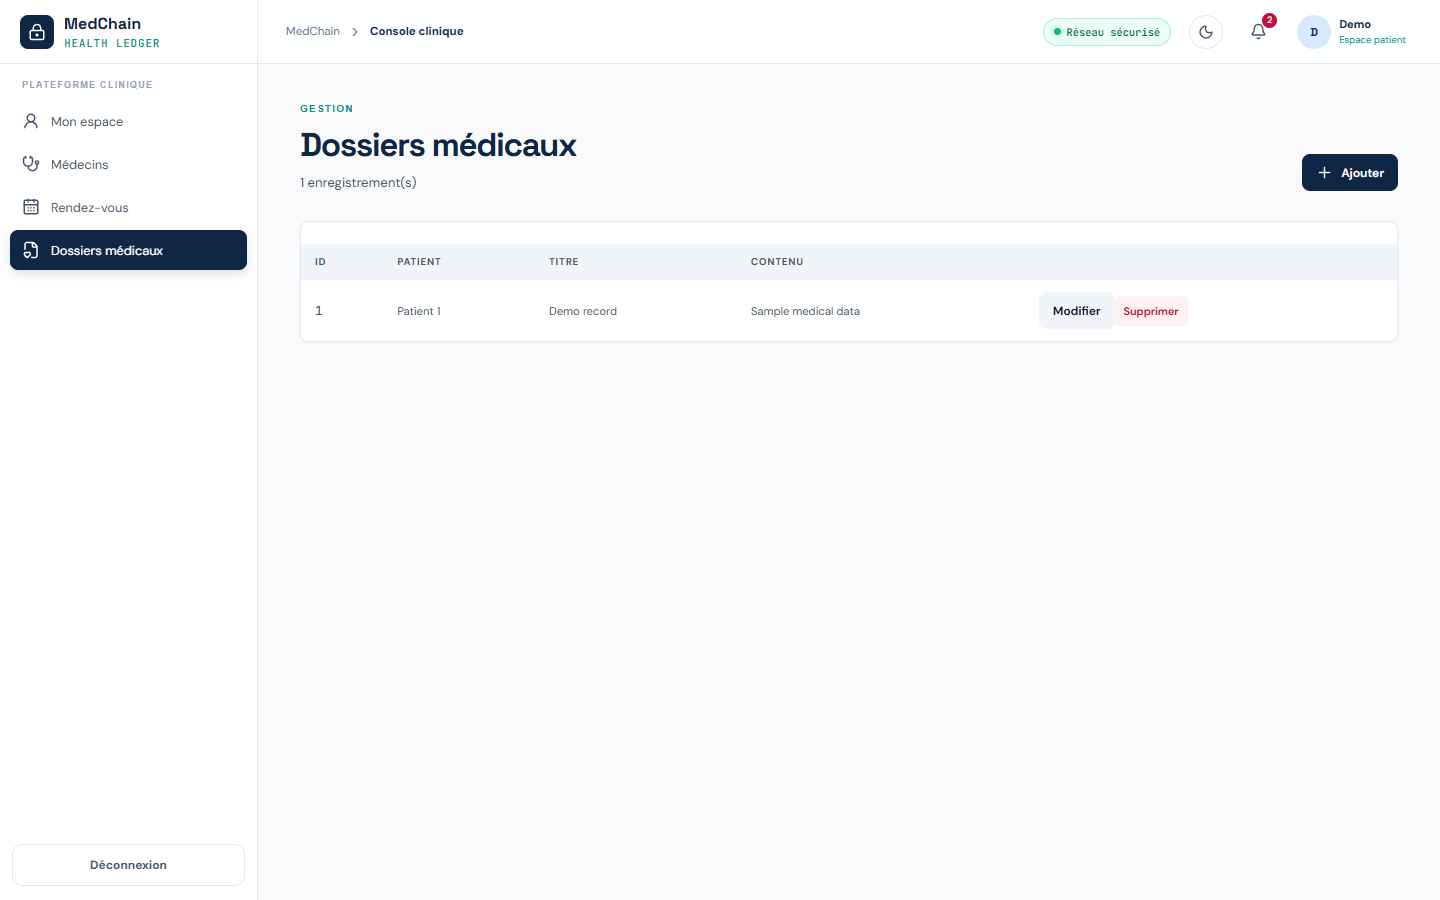
\includegraphics[width=\textwidth]{S09-liste-dossiers.png}
\caption{Liste des dossiers médicaux}
\label{fig:records}
\end{figure}

\section{Réalisation --- Espace médecin}

La Figure \ref{fig:doctor_dash} montre l'espace médecin et la Figure \ref{fig:patients_list} la liste des patients. La Figure \ref{fig:event_form} détaille la timeline d'un épisode et le formulaire d'ajout d'un événement clinique.

\begin{figure}[H]
\centering
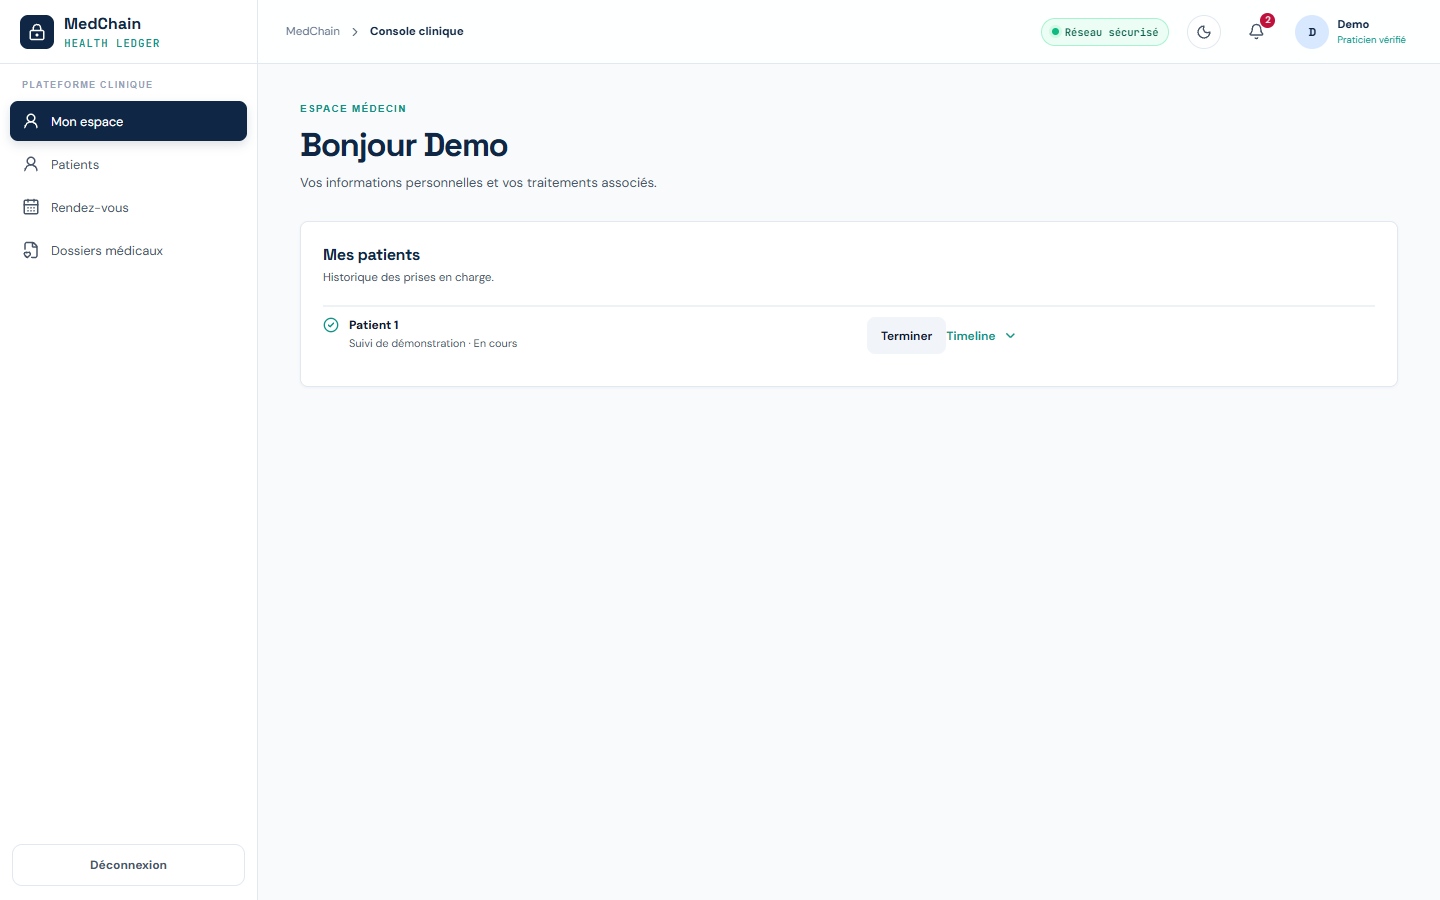
\includegraphics[width=\textwidth]{S11-espace-medecin.png}
\caption{Tableau de bord médecin}
\label{fig:doctor_dash}
\end{figure}

\begin{figure}[H]
\centering
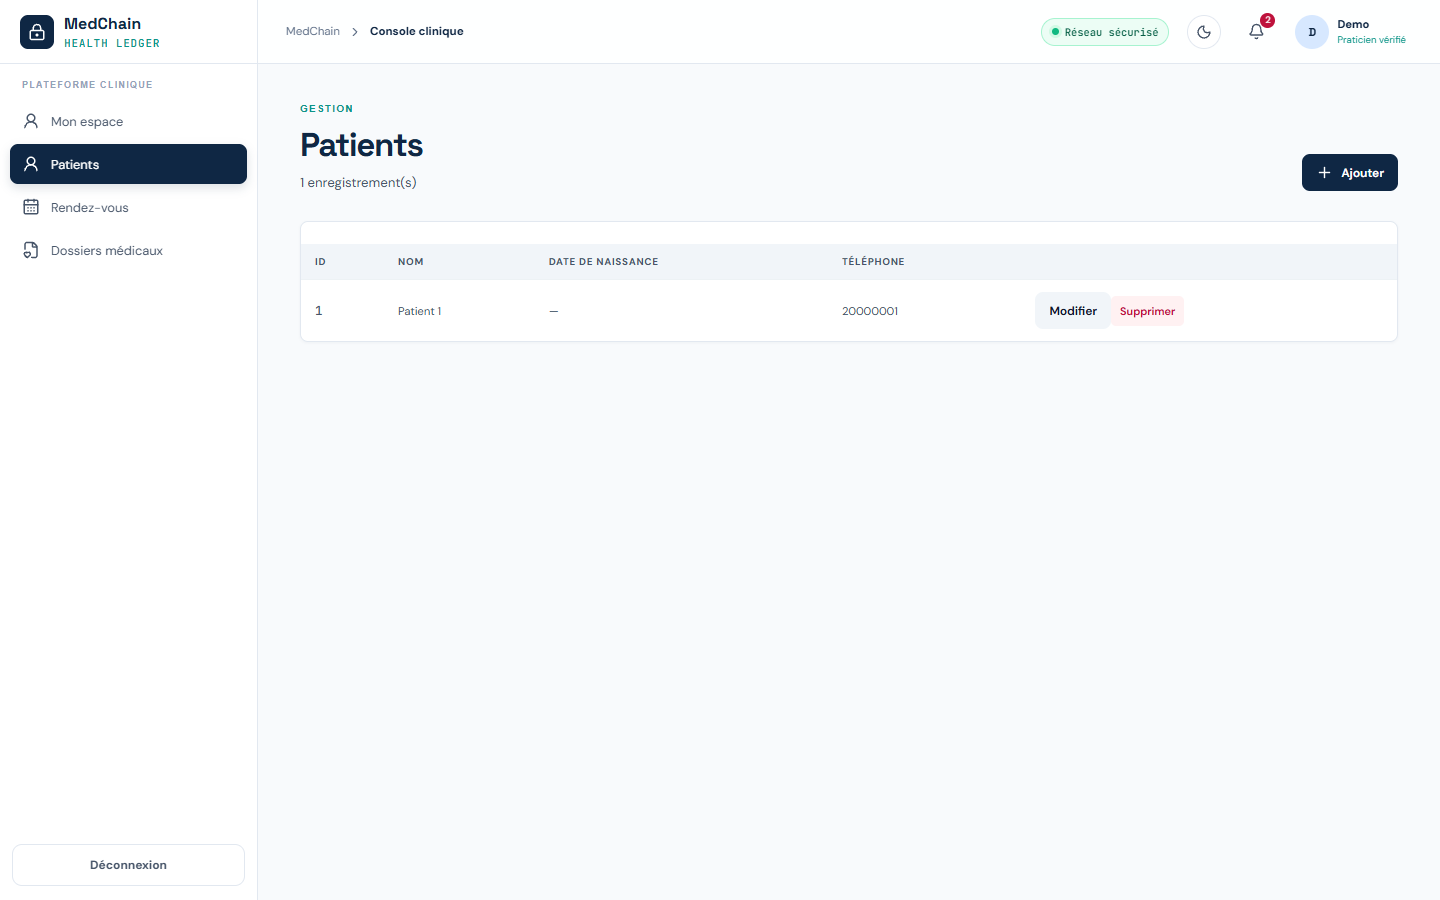
\includegraphics[width=\textwidth]{S12-liste-patients.png}
\caption{Liste des patients}
\label{fig:patients_list}
\end{figure}

\begin{figure}[H]
\centering
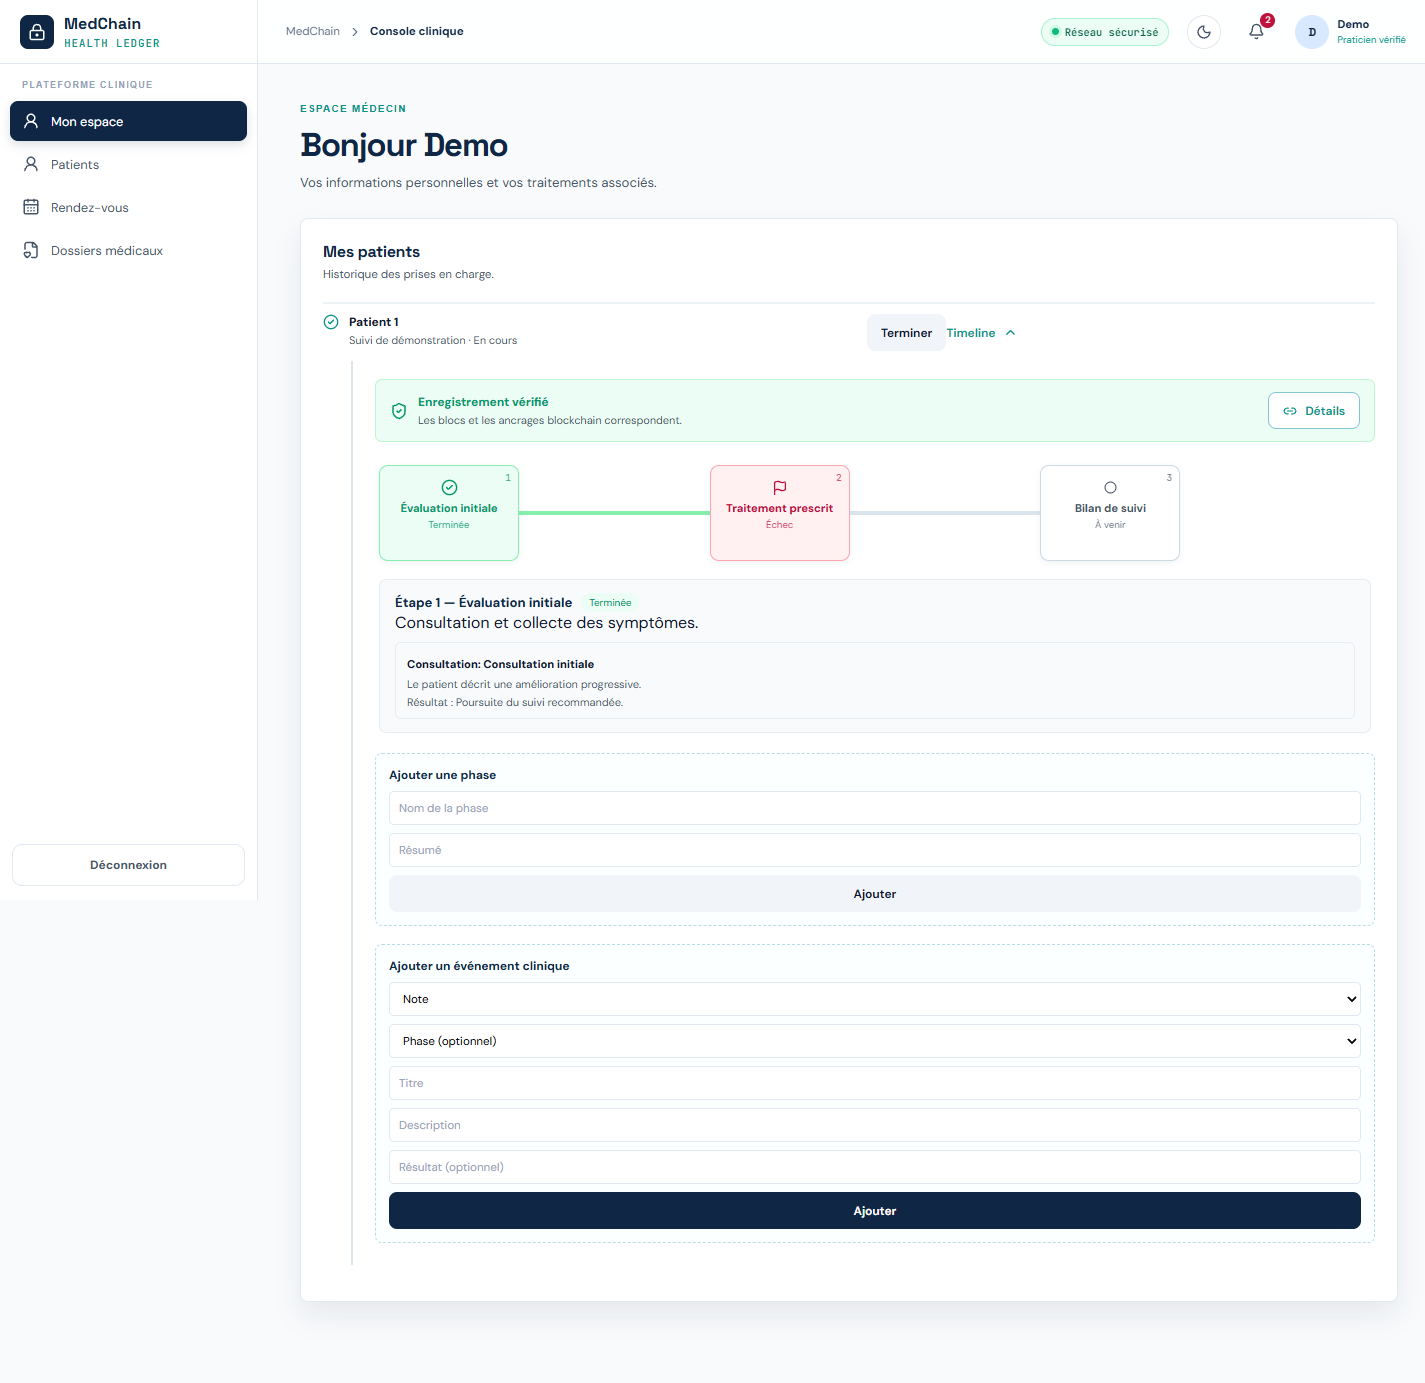
\includegraphics[width=\textwidth]{S13-ajout-evenement-traitement.png}
\caption{Timeline et ajout d'un événement clinique}
\label{fig:event_form}
\end{figure}

\section{Conclusion}

Le parcours de soins est désormais couvert de bout en bout, avec une visualisation de l'état d'intégrité directement dans l'interface. Le chapitre suivant décrit le chiffrement, la formation des blocs et l'ancrage.

\chapter{Sprint 3 : Sécurité, chiffrement et supervision}\label{chap6}

\section{Introduction}

Le troisième sprint renforce la confidentialité des données cliniques et la preuve d'intégrité. Chaque événement de traitement est chiffré avec une clé de données propre à l'épisode, puis son empreinte est inscrite dans deux chaînes de blocs et ancrée sur une chaîne EVM locale.

\section{Chiffrement enveloppe}

La Figure \ref{fig:envelope} présente le mécanisme de chiffrement. Une clé maître, fournie par l'environnement, dérive une clé d'encapsulation (KEK). Une clé de données (DEK) aléatoire est générée par épisode, encapsulée par la KEK et stockée dans \texttt{EpisodeKey}. La charge utile de l'événement est chiffrée avec la DEK puis conservée dans \texttt{Block.payload\_enc}.

\begin{figure}[H]
\centering
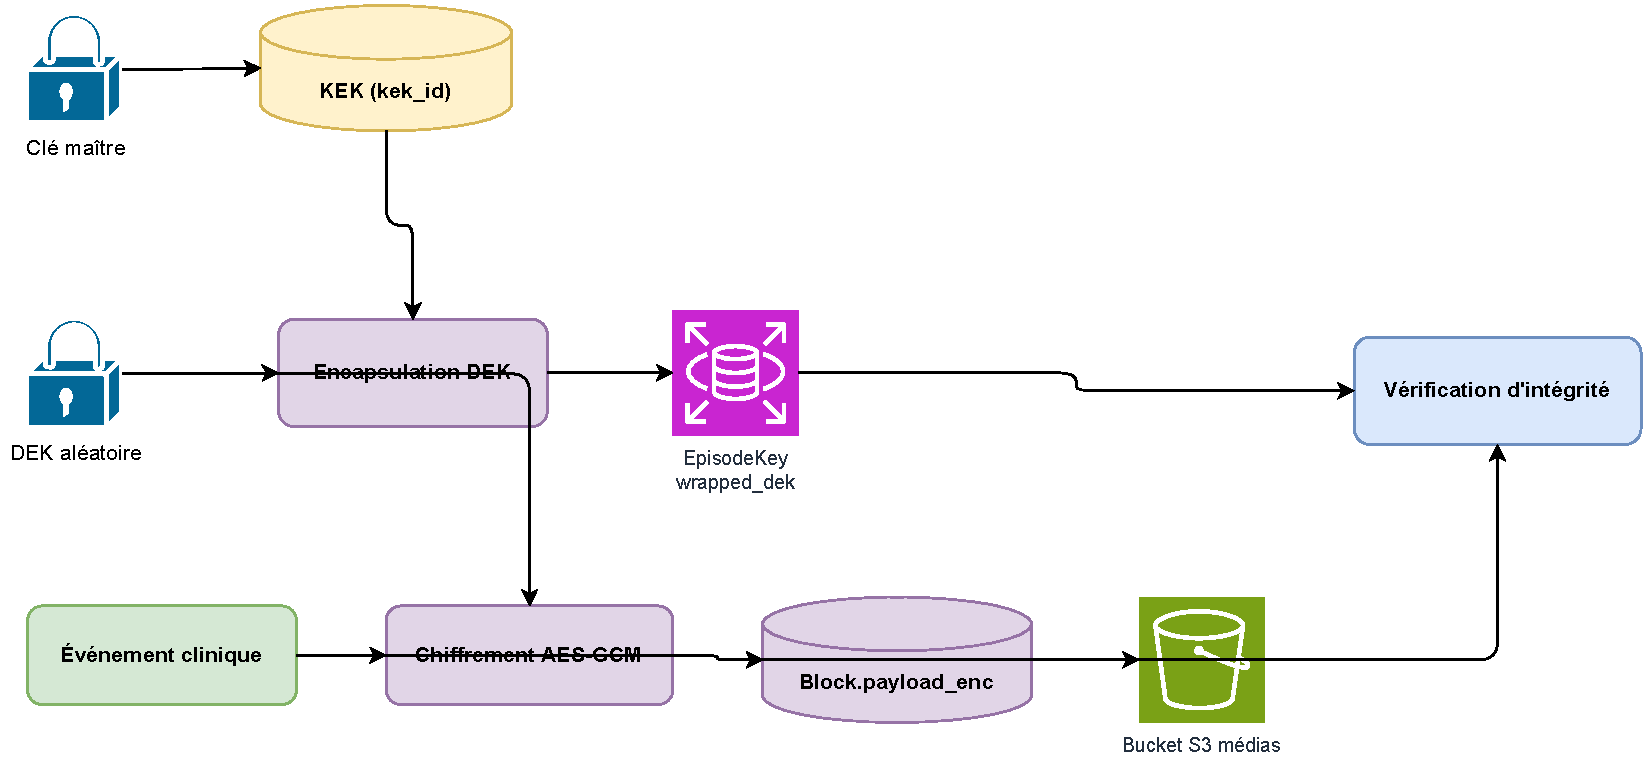
\includegraphics[width=\textwidth]{10-chiffrement-enveloppe.pdf}
\caption{Flux de chiffrement enveloppe}
\label{fig:envelope}
\end{figure}

Cette conception permet de séparer les responsabilités : la base stocke des octets chiffrés, le fournisseur de clés reste externalisé, et la rotation de la clé maître peut être organisée sans réécrire les événements passés.

\section{Formation et ancrage des blocs}

La Figure \ref{fig:chain_seq} décrit la séquence complète. Après création de l'événement, le système calcule une empreinte et une racine Merkle, crée un bloc immuable dans la chaîne du patient ou du médecin, puis envoie le hash du bloc à Anvil. La transaction d'ancrage et le numéro de bloc sont conservés dans \texttt{Anchor}.

\begin{figure}[H]
\centering
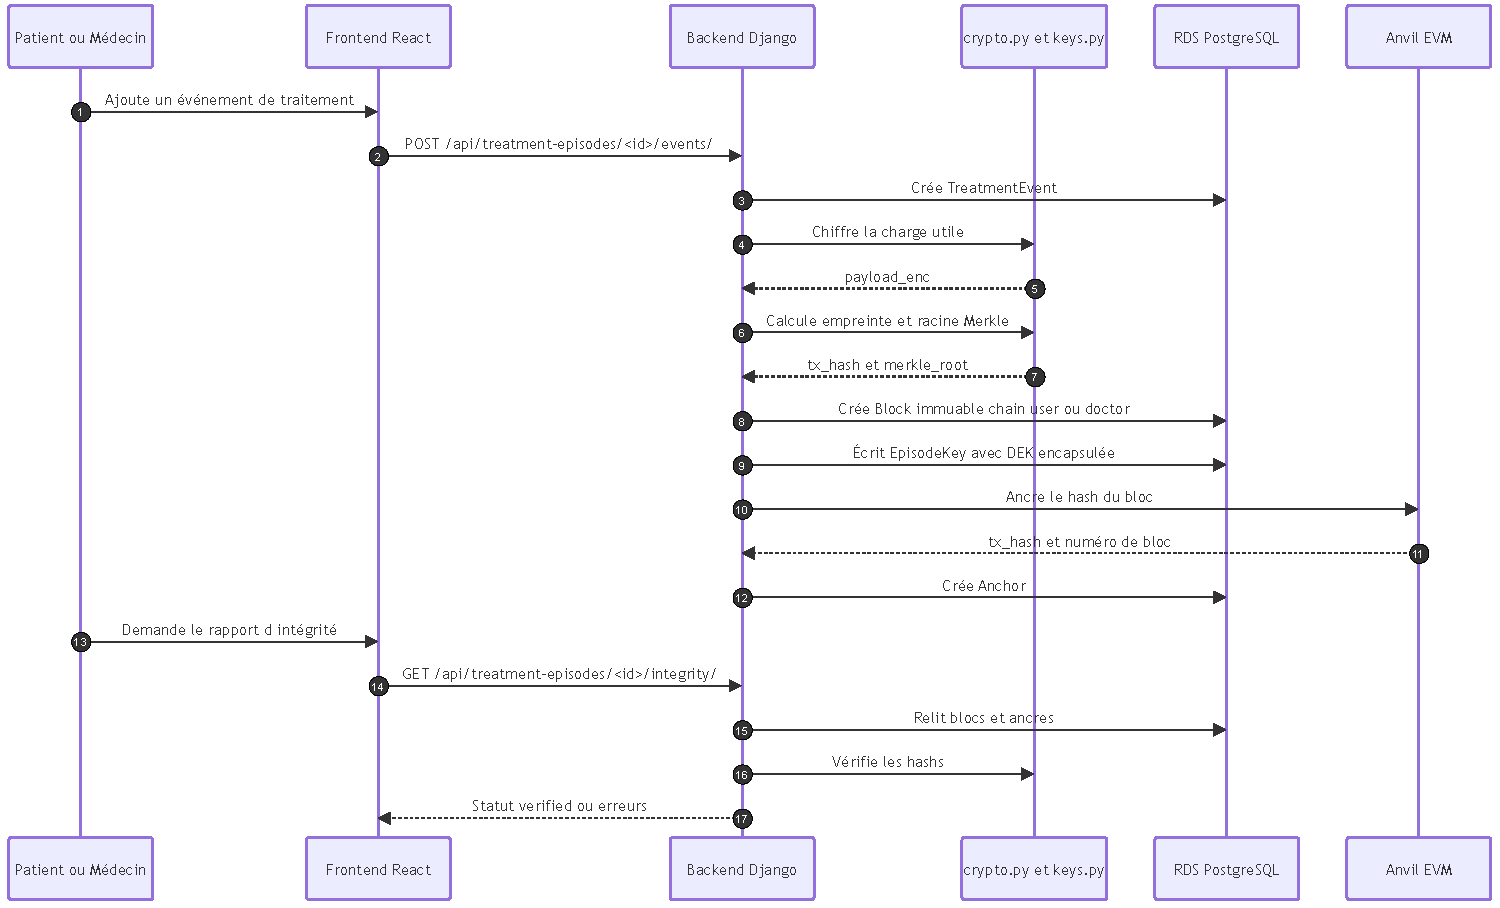
\includegraphics[width=\textwidth]{09-integrite-blockchain-sequence.pdf}
\caption{Séquence d'intégrité et d'ancrage blockchain}
\label{fig:chain_seq}
\end{figure}

Le modèle \texttt{Block} interdit toute modification ou suppression : les méthodes \texttt{save} et \texttt{delete} lèvent une exception dès que l'objet possède une clé primaire. Les blocs sont organisés en deux chaînes par épisode, chacune avec un index unique et un hash du bloc précédent.

\section{Supervision et journaux}

La Figure \ref{fig:logs} montre le pipeline de journalisation. Le backend émet des JSON structurés avec un identifiant \texttt{X-Request-ID}. Fluent Bit collecte ces flux, les enrichit et les envoie à Elasticsearch, où Kibana permet de construire des tableaux de bord et des alertes.

\begin{figure}[H]
\centering
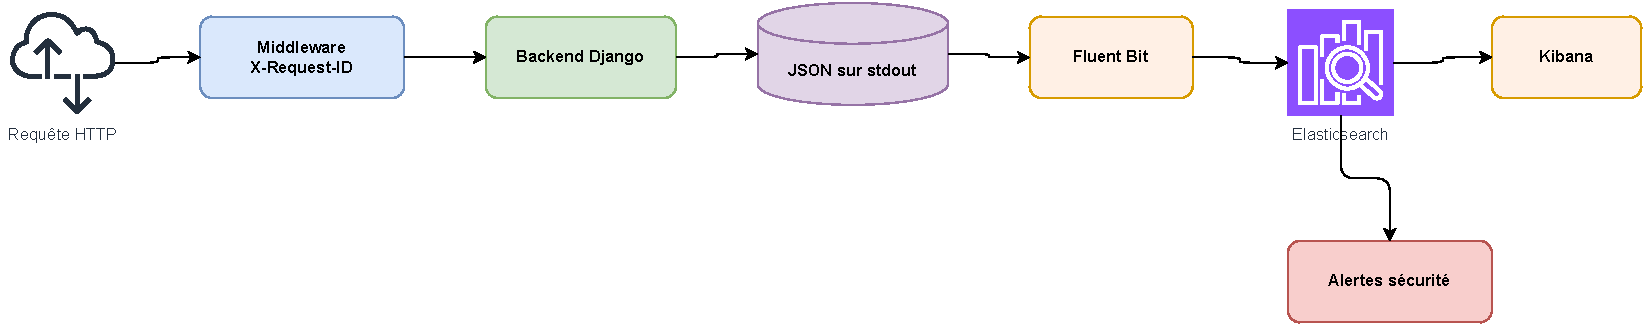
\includegraphics[width=\textwidth]{11-pipeline-logs.pdf}
\caption{Pipeline de collecte et d'analyse des journaux}
\label{fig:logs}
\end{figure}

La Figure \ref{fig:audit} illustre la vue administrateur qui donne accès aux utilisateurs, aux alertes de sécurité et aux dernières activités.

\begin{figure}[H]
\centering
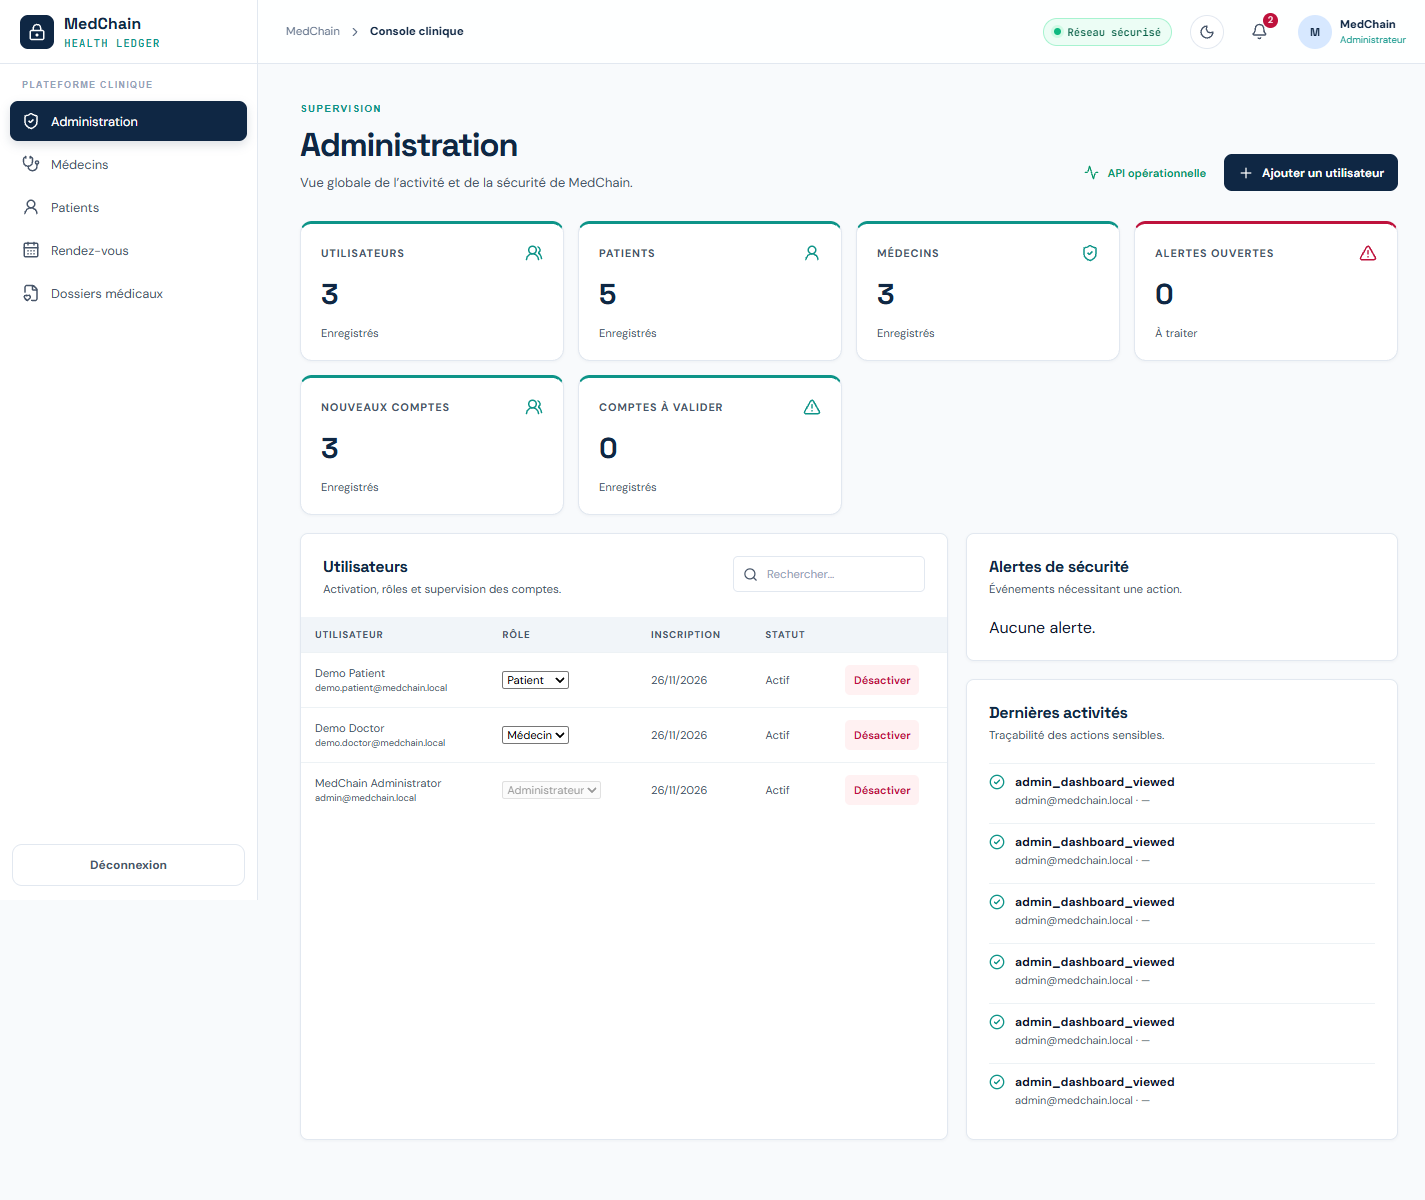
\includegraphics[width=\textwidth]{S15-audit-et-alertes.png}
\caption{Journal d'audit et alertes de sécurité}
\label{fig:audit}
\end{figure}

\section{Conclusion}

Le volet sécurité est désormais complet : chiffrement des charges utiles, immutabilité des blocs, ancrage des empreintes et supervision des accès. Le dernier chapitre présente le déploiement et les résultats de validation.

\chapter{Déploiement, validation et conclusion}\label{chap7}

\section{Architecture de déploiement}

La Figure \ref{fig:deploy} présente la topologie des services. En local, Docker Compose orchestre la passerelle Nginx, le frontend React servi par Nginx, le backend Django sous Gunicorn, PostgreSQL, Redis, la chaîne Anvil, Fluent Bit, Elasticsearch et Kibana. Les healthchecks imposent l'ordre de démarrage : la base puis le backend, et enfin le frontend.

La cible d'exécution retient une base PostgreSQL managée (\textbf{RDS}) comme stockage par défaut et un \textbf{bucket S3} pour les fichiers médias. La configuration Django conserve le moteur PostgreSQL via les variables \texttt{DB\_*} et le backend de stockage via \texttt{STORAGE\_BACKEND}, ce qui rend le changement de service transparent pour le code applicatif.

\begin{figure}[H]
\centering
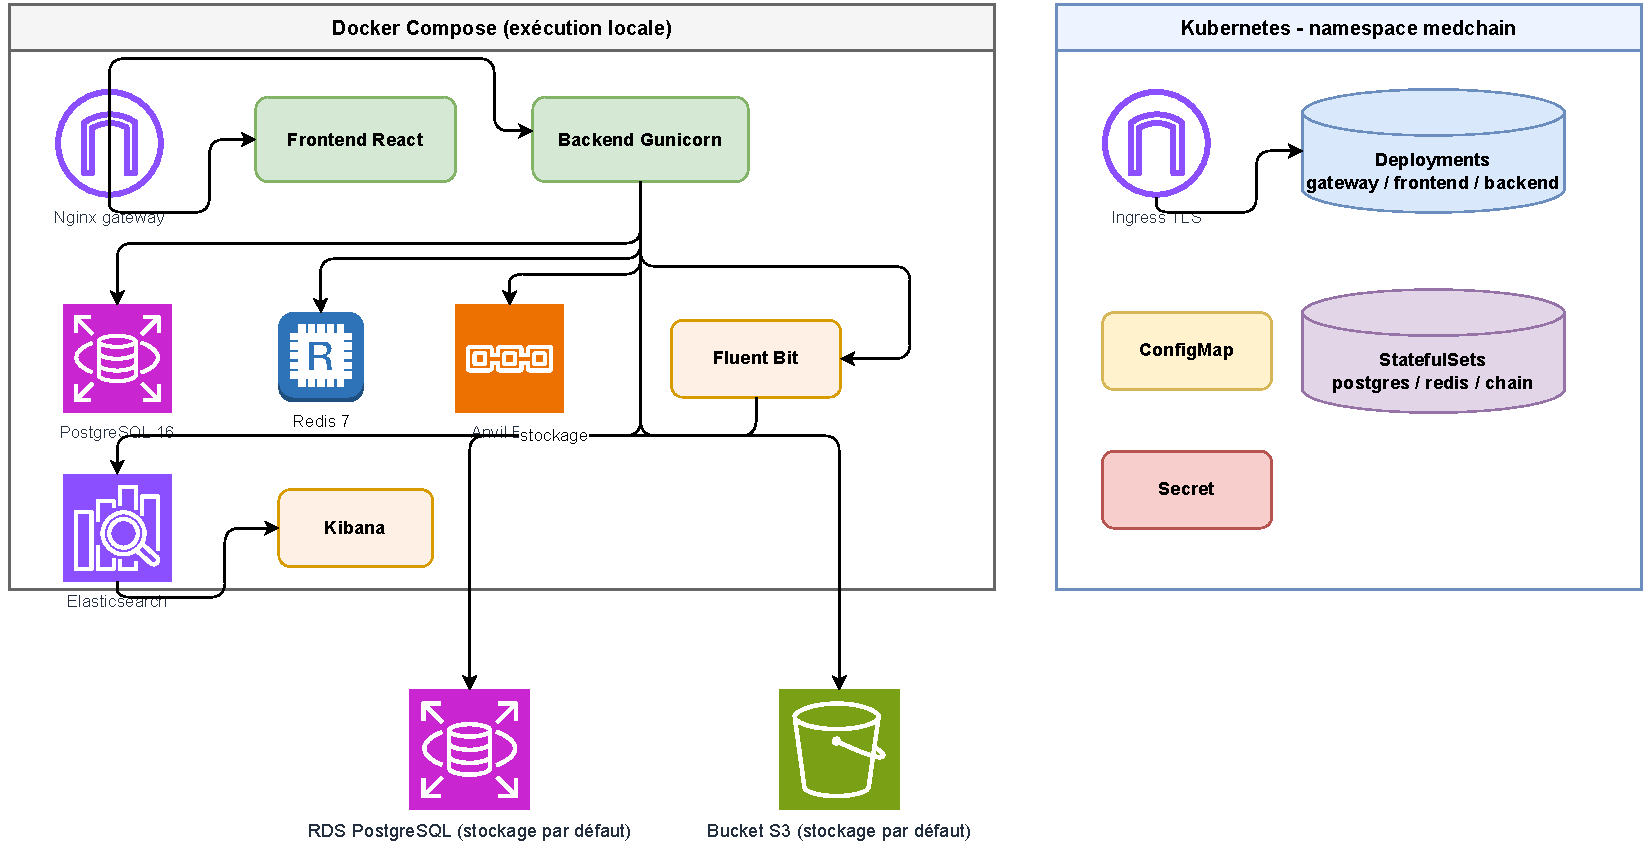
\includegraphics[width=\textwidth]{03-topologie-deploiement.pdf}
\caption{Topologie de déploiement locale et cible}
\label{fig:deploy}
\end{figure}

\section{Conteneurisation et Kubernetes}

Chaque service possède image, variables d'environnement et healthcheck explicites. Les manifestes Kubernetes du namespace \texttt{medchain} complètent cette base avec un Ingress TLS, une ConfigMap, des Secrets, des volumes persistants et une séparation des composants de journalisation facultatifs.

\section{Validation fonctionnelle}

La validation a porté sur les points suivants :

\begin{itemize}
    \item construction des images backend et frontend ;
    \item connexion du backend à la base et exécution des migrations ;
    \item authentification d'un compte patient, d'un compte médecin et d'un compte administrateur ;
    \item appel d'une route protégée avec le jeton retourné ;
    \item vérification du filtrage des épisodes selon le rôle ;
    \item consultation de la timeline et des détails d'intégrité ;
    \item ancrage des blocs sur la chaîne locale et lecture des transactions ;
    \item service du frontend par la passerelle et accès à la documentation OpenAPI.
\end{itemize}

La Figure \ref{fig:swagger} illustre la documentation interactive générée automatiquement à partir du schéma OpenAPI.

\begin{figure}[H]
\centering
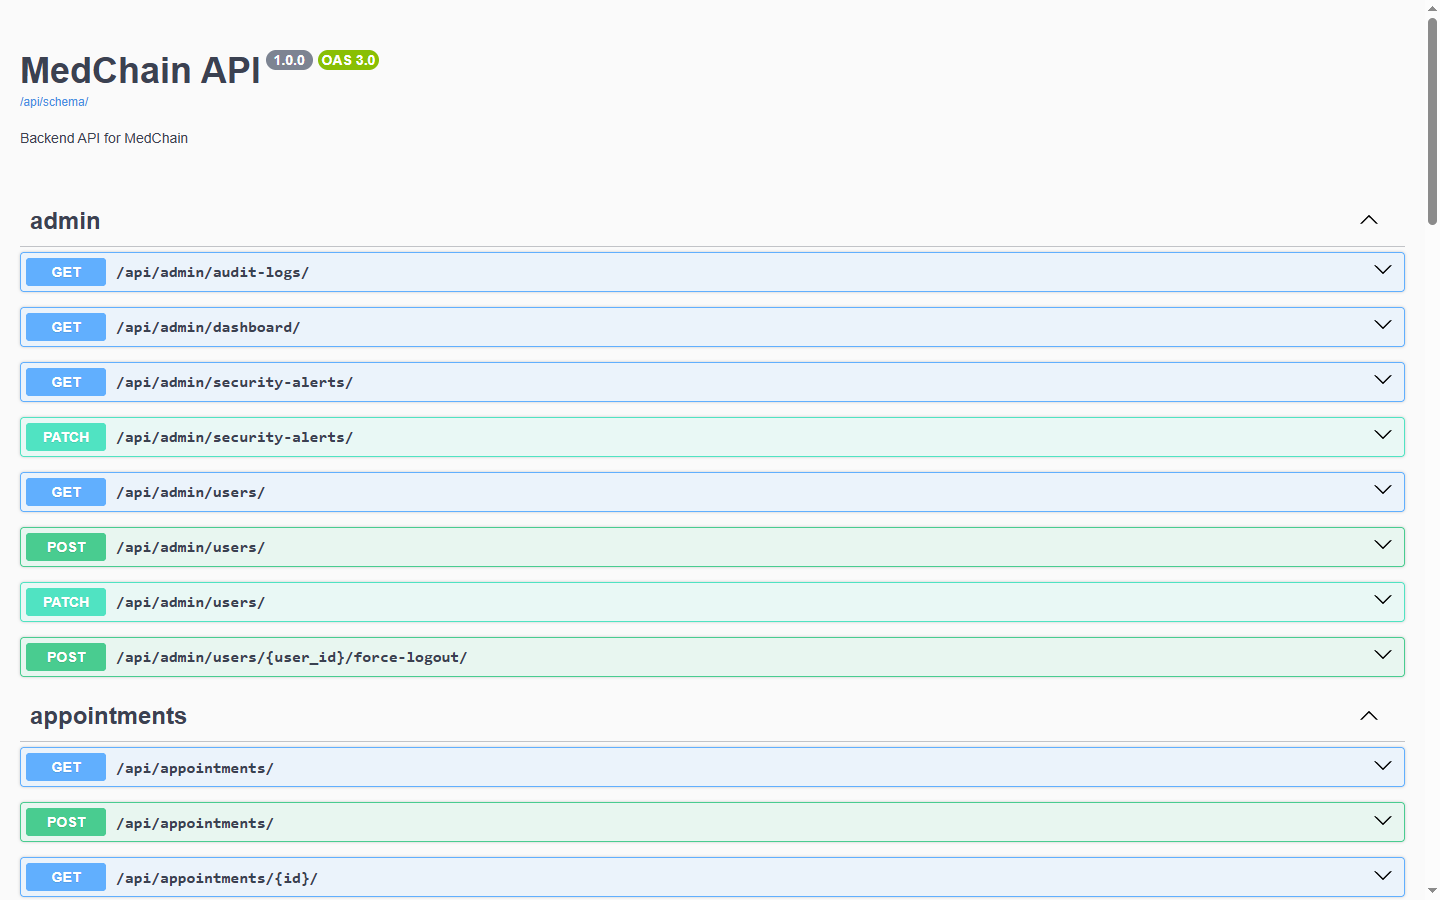
\includegraphics[width=\textwidth]{S16-swagger-api.png}
\caption{Documentation interactive de l'API}
\label{fig:swagger}
\end{figure}

\section{Limites et perspectives}

Certaines évolutions restent à réaliser :

\begin{itemize}
    \item remplacer le fournisseur de clés basé sur l'environnement par un service de gestion de clés externe ;
    \item migrer l'ancrage local vers un registre public ou une infrastructure de production ;
    \item durcir les déploiements Kubernetes avec des politiques réseau et des quotas de ressources ;
    \item compléter la couverture de tests sur les scénarios d'accès refusé ;
    \item industrialiser le pipeline d'intégration continue avec analyse de sécurité des dépendances.
\end{itemize}

\section{Conclusion générale}

MedChain démontre qu'il est possible de concilier confidentialité et vérifiabilité dans un dossier médical partagé. Le chiffrement enveloppe protège le contenu, l'immutabilité des blocs et l'ancrage garantissent l'intégrité de l'historique, et le filtrage par rôle limite l'exposition des données. L'architecture conteneurisée et la séparation configuration/secrets fournissent une base pour un passage à l'échelle vers RDS et S3.


%%% Glossaire %%%
\printglossaries

%%% Bibliographie %%%
\chapter*{Bibliographie}
\addcontentsline{toc}{chapter}{Bibliographie}
\begin{enumerate}
\item Django REST Framework, \url{https://www.django-rest-framework.org/}
\item React, \url{https://react.dev/}
\item Nginx, \url{https://nginx.org/en/docs/}
\item PostgreSQL, \url{https://www.postgresql.org/docs/}
\item Amazon Web Services, \url{https://docs.aws.amazon.com/}
\item Web3.py, \url{https://web3py.readthedocs.io/}
\item draw.io, \url{https://www.drawio.com/doc/}
\end{enumerate}

%%% Webographie %%%
\chapter*{Webographie}
\addcontentsline{toc}{chapter}{Webographie}
\begin{enumerate}
\item \textbf{Django} --- \url{https://www.djangoproject.com/} : framework backend et ORM.
\item \textbf{DRF Spectacular} --- \url{https://drf-spectacular.readthedocs.io/} : génération du schéma OpenAPI.
\item \textbf{React Router} --- \url{https://reactrouter.com/} : routage de l'application monopage.
\item \textbf{Docker Compose} --- \url{https://docs.docker.com/compose/} : orchestration locale des services.
\item \textbf{Kubernetes} --- \url{https://kubernetes.io/docs/} : manifests de déploiement du namespace medchain.
\item \textbf{Elasticsearch et Kibana} --- \url{https://www.elastic.co/guide/} : collecte et visualisation des journaux.
\item \textbf{Anvil} --- \url{https://book.getfoundry.sh/anvil/} : chaîne EVM locale pour les tests d'ancrage.
\end{enumerate}

\end{document}
